% This template has been downloaded from:
% http://www.LaTeXTemplates.com



%----------------------------------------------------------------------------------------
%PACKAGES AND OTHER DOCUMENT CONFIGURATIONS
%----------------------------------------------------------------------------------------

\documentclass[oneside]{article}
\usepackage{multicol}

\usepackage{lipsum} % Package to generate dummy text throughout this template


\usepackage[T1]{fontenc} % Use 8-bit encoding that has 256 glyphs


\usepackage[hmarginratio=1:1,top=32mm,columnsep=20pt]{geometry} % Document margins
%\usepackage{multicol} % Used for the two-column layout of the document
\usepackage[hang, small,labelfont=bf,up,textfont=it,up]{caption} % Custom captions under/above floats in tables or figures
\usepackage{booktabs} % Horizontal rules in tables
\usepackage{float} % Required for tables and figures in the multi-column environment - they need to be placed in specific locations with the [H] (e.g. \begin{table}[H])
\usepackage{hyperref} % For hyperlinks in the PDF
\usepackage{listings}
\usepackage{url}
\usepackage{graphicx}
\usepackage{wrapfig}
\usepackage[table,xcdraw]{xcolor}
\usepackage{caption}
\usepackage{pdfpages}
\usepackage{tabu}
\usepackage{longtable}
%\graphicspath{ {image/} }

\usepackage{lettrine} % The lettrine is the first enlar ed letter at the beginning of the text
\usepackage{paralist} % Used for the compactitem environment which makes bullet points with less space between them

%\usepackage{abstract} % Allows abstract customization
%\renewcommand{\abstractnamefont}{\normalfont\bfseries} % Set the "Abstract" text to bold
%\renewcommand{\abstracttextfont}{\normalfont\small\itshape} % Set the abstract itself to small italic text


\usepackage{titlesec} % Allows customization of titles
\renewcommand\thesection{\arabic{section}} % Arabic numerals for the sections
\renewcommand\thesubsection{\arabic{section}.\arabic{subsection}} % Arabic numerals for subsections
\titleformat{\section}[block]{\large\scshape\centering}{\thesection}{1em}{} % Change the look of the section titles
\titleformat{\subsection}[block]{\large}{\thesubsection}{1em}{} % Change the look of the section titles

\usepackage{fancyhdr} % Headers and footers
\pagestyle{fancy} % All pages have headers and footers
\fancyhead{} % Blank out the default header
\fancyfoot{} % Blank out the default footer
%\fancyhead[C]{Running title $\bullet$ November 2012 $\bullet$ Vol. XXI, No. 1} % Custom header text
\fancyfoot[RO,LE]{\thepage} % Custom footer text

%----------------------------------------------------------------------------------------
%TITLE SECTION
%----------------------------------------------------------------------------------------
\begin{document}

\begin{titlepage}

\newcommand{\HRule}{\rule{\linewidth}{0.5mm}}
\center
\textsc{\LARGE King's College London}\\[1.5cm]
\textsc{\Large Traffic Simulator Group Project - 7CCSMGPR}\\[0.5cm]
%\textsc{\large Group Project}\\[0.5cm]
\HRule \\[0.4cm]
{ \huge \bfseries Stuck In Traffic}\\[0.4cm]
\HRule \\[1.5cm]

\begin{minipage}{0.4\textwidth} \large
\begin{center}
%\emph{Members:}\\
Antria Dimitriou \\
Filippo Mariani \\
Maximilian Nikolaidis \\
Filippos Raditsas \\
Maxim Vasilishin
\end{center}
\end{minipage}
\\[1cm]


\includegraphics{King's_College_London_crest}\\[1cm] 

%{\large \today}\\[3cm]

\vfill

\end{titlepage}

%\title{\vspace{-20mm}\fontsize{20pt}{10pt}\selectfont\textbf{Stuck in Traffic Final Project Report}}
%\author{
%\large
%{Antria Dimitriou, Filippo Mariani, Maximilian Nikolaidis, Filippos Raditsas, Maxim Vasilishin}\\[10mm] % Your name
%\normalsize King's College London \\ [50mm] % Your institution
%\normalsize {\textit{7CCSMGPR Group Project: Traffic Management Simulation}}
%%\normalsize \href{mailto:filippo.mariani@kcl.ac.uk}{filippo.mariani@kcl.ac.uk} % Your email address
%\vspace{-85mm}
%}
%\date{}
%%
\clearpage
%


%






%----------------------------------------------------------------------------------------



%\lhead{\emph{Contents}} % Set the left side page header to "Contents"
\tableofcontents % Write out the Table of Contents
%\clearpage

%\lhead{\emph{List of Figures}} % Set the left side page header to "List of Figures"
\listoffigures % Write out the List of Figures
%\clearpage

%\lhead{\emph{List of Tables}} % Set the left side page header to "List of Tables"
\listoftables % Write out the List of Tables
\clearpage

%\maketitle %add title

%\thispagestyle{fancy} % All pages have headers and footers

%----------------------------------------------------------------------------------------
%ABSTRACT
%----------------------------------------------------------------------------------------

%\begin{abstract}

%\noindent \lipsum[0]  % Dummy abstract text

%\end{abstract}

%\clearpage 
%----------------------------------------------------------------------------------------
%ARTICLE CONTENTS
%----------------------------------------------------------------------------------------

%\begin{multicols}{2} % Two-column layout throughout the main article text


\section{Introduction}

Traffic management is a well-known problem within metropolitan cities, such as London. There are a number of increasing factors we need to take into account in order to tackle traffic management, these factors make it even more complicated. Throughout the years, a great amount of research has been invested in the area of improving traffic management, in which the outcome to be most efficient and easy to use systems. Environmental factors, such as energy consumption \cite{macneille2013integration, 5973655, osorio2013energy} and pollution levels \cite{panis2006modelling}, along with vehicle to vehicle communication \cite{conceiccao2008large}, are some examples of major research topics in the area of traffic optimization. Inspired by the variety of different approaches of the general problem, our idea was to ultimately create a fully customizable simulation engine. Our vision was to provide a simulator to users wishing to perform traffic simulations to observe certain scenarios and come up with potential solutions in their research. An engine that would also be fully extensible by developers \& researchers that wish to take a different approach. As a result, we have decided to begin a project entirely from scratch, without the use of any external libraries, or any existing tools.\\
\newline
\noindent Our aspiration for this simulation engine is to provide the user with an intelligent, easy to use software, as well as accommodating developers with an engine upon which they can implement their ideas and further customize the software accordingly. However, due to the time constraints, as well as the requirements of the Group Project module to come up with a traffic simulation engine, we implemented it to be more focused to the traffic management aspect. We accomplished to build an independent and extensible simulation engine, that integrates with a map builder, a Graphic User Interface(GUI), and different agents. The simulation engine is also able to gather data from all the activity and other components (e.g. maps, agents) in the simulation and generate reports. For example a report could contain information such as the average car speed, simulation speed, simulation duration, etc. Unfortunately, due to the time limits, even though we have implemented the capabilities of the simulation engine to generate reports, we have not presented all of the possible reports in the simulation. More specifically, there are information of the simulation available from which we can generate more comprehensive reports to the users but due to the time limitations we haven't implemented it. Furthermore, our map builder offers customizable grid size, different types of roads for the users to choose from, in order to build their maps, and the ability to save and load maps to and from the users' computer file system. 
\newline

\noindent In order to develop this solution we implemented a traffic simulator that allows users to simulate the most common scenarios that can be experienced during a normal day. For this reason, many different types of roads have been included, along with different agents (cars, traffic lights, etc.). The simulator, among other features, is able to reproduce a scenario where two or more vehicles meet at an intersection, and we will simulate how the traffic lights will handle such scenarios to control traffic flow. One of our solution's capabilities is to provide users with an initial understanding of the problem faced by road traffic enforcement and optimization. The simulation will try to provide a solid starting block to further simulations and observations, this will allow users to create their own maps. Upon initialization of our simulator and the choice of a map, all possible paths are going to be calculated and all the cars entering the grid will have predefined randomly chosen starting and ending point as well as a path that they will follow. Further details on the requirements we have set and technical details regarding the implementation are going to be discussed later on in this report.
\newline

\noindent The report is organized as follows: Section 2 provides an overview of related traffic simulation projects that has helped us understand and define the requirements for our traffic simulation. Section 3 we specify the requirements that we have set, along with the limitations and the reasons we set those requirements, as well as an overview of the project description. Section 4 we provide details of the implementation, in this chapter we will discuss in detail the software simulator and the most important functionalities, problems faced, and there solutions. Section 5 describes activities related to team work and how we used different tools and processes to efficiently collaborate during the project development. Section 6 will present an overall project evaluation and propose some ideas regarding future work, as well as optimization of our existing software solution. Ultimately, in section 7 we will present a table depicting peer assessment within our team.
\newpage

\section{Review}

The object of interest in this section is to review related developments and tools for traffic simulation systems. The related work in similar projects is available in the traffic management industry, most of the pre-existing projects have used open-source software for multi-agents simulation for their development. Naturally, existing software will either outperform or lag regarding the objectives of our project. This kind of software may differ from other's work in many aspects such as: 2-dimensional or 3-dimensional representation, quality of graphics, types of vehicles (cars, buses, taxis, long vehicles), traffic lights, types of roads (horizontal and vertical roads, intersection, single or double lane roads, roundabout, one-way road), external factors (parking slots, pedestrians, crossings), behaviour of drivers (intelligence system), road works and much more. 
\newline

\noindent There are many open-source tools available in the market for developing simulation systems and traffic modelling; some of them are Aimsun, TransModeler \cite{TransModeler}, RoadTrafficSimulator, AnyLogic, SUMO etc. In paper \cite{jones2004traffic}, three tools are compared (AIMSUN, CORSIM and SimTraffic) and shows that all three are able to provide reasonable results for typical simulation software. Certainly, project limitations and planning analysis should be considered before selecting the appropriate tool. All of the tools are available to help developing a simulation software, though each tool package can display strengths and weaknesses depending on developers' preferences; packages can include microscopic, macroscopic and mesoscopic simulations models. Although Aimsun is one of the most famous simulation and modelling software tools which has been integrated by TSS and many high-level projects have been developed with the help of Aimsun \cite{auss}. Additionally, in 2010 a well-developed model is presented and successfully handles lane changes and traffic behaviours based on different speed limits in order to have a scalable and interactive system for real-time scenarios \cite{sewall2010continuum}. This method has been developed using the open-source traffic simulation package, SUMO, and it has been tested and proved that it can work on large, real-world road networks. SUMO techniques and characteristics are discussed further in \cite{kotusevski2009review} where it is compared with other simulation tools. Even the mentioned tools can make software's developers life much easier in both coding and graphics development, we haven't used anything similar since we wanted our project to be built from scratch.
\newline

\noindent Although, a micro-simulation model is available online which presents and executes a roundabout simulation where the traffic is controlled based on the speed and type of the cars (fast/slow, normal car/long vehicle) by using html5 and JavaScripts\cite{traffichtml5}. The mentioned example was a good guidance for getting a visual idea of how the entire system will manage the traffic. In \cite{yang2000simulation}, a high-level laboratory environment is generated for representing microscopic traffic simulator and a traffic management simulator. It is actually a computer based simulation laboratory for evaluating dynamic traffic management systems. Imagine a computer-based side which is controlled by humans where their system is connected with a microscopic traffic simulator attached in real-life roads. This project has been developed using C++ object-oriented programming language and it contains a graphical user interface which allows the user to have a visual simulation as our project is indented to do. Furthermore, in paper \cite{luke2005mason}, we have identified a model that is partially related with our project objective since it introduces a multi-agent simulation toolkit developed using Java programming tool. MASON, as the creators named it, was designed to serve the basis of multi-agent simulation tasks such as from swarm robotics to machine learning to social environments. The aim of this project is to make its use easy to be modified in both programming and graphical representation. MASON has the ability to keep separately the model from the visualization dynamically or to reattach the simulation to another platform in the middle of the run. 
\newline

\noindent In 2006, a modelling technique is presented to describe the behaviour of urban traffic systems by having as a case study a real intersection in a city of Italy, called Bari \cite{dotoli2006urban}. The traffic network model has been generated by using the mathematical modelling language Petri Nets and the Coloured Timed Petri Net(CTPN) for describing the flow of vehicles. The idea behind this modelling technique is to show that a Petri Net model can be easily translated to traffic control simulation software with the appropriate programming skills but without any significant costs.
\newline

\noindent Traffic has been and will continue to be a serious problem for drivers in both small towns and large cities. Thus, in 1999 a system of intersection controllers in traffic lights is described \cite{tavladakis1999development}. An area-wide traffic control system is presented by using predictions to test and control the functionality of the traffic lights in intersections. This system is considered as a cyclic system since the results taken from a current cycle (execution), and they are then used to test the behaviour of the system for the next cycle. The system can only be used to control the traffic in isolated nodes as well as in the centre of small towns but it cannot handle large and demanding roads. 
\newline

\noindent In 2011 the creators of an intelligent traffic light system focus on three test cases, which are empty street case, normal street case and crowded street case and they are proposed as an additional component for improving the traffic light configuration \cite{kareem2011intelligent}. This case can be related with our project since we have the functionality of increasing the number of cars in the simulation phase. The empty street case is where few or zero cars are on the map, normal street case is where number of cars corresponds to the size of the grid and not too many cars are on the map thus the possibility of being stuck in traffic is eliminated. Last but not least, it is the overcrowded street case where the user can add the maximum number of cars that the grid can accept resulting in traffic congestion, this is where the traffic simulator is the most important. 
\newline

\noindent In addition, software developers introduce an intelligent system that has been built for monitoring and controlling the flow of traffic using Java programming language \cite{chinyere2011design}. They have used the methodology of Fuzzy Logic which is an approach based on truth and logic statements instead of the usual Boolean logic used in the most modern computers, true or false (0 or 1) \cite{fuzzyLogic}. The software was simulated and tested for a popular intersection in a city in Nigeria to control the flow of the traffic in order to show its efficiency. The objective of this paper matches with the objective of our project, where dynamic software has been developed to be as efficient as well as user-friendly software regardless the complexity of the software. The content of the project evolving in \cite{center1996intelligent} is based again in fuzzy logic technology which has been built to implement an intelligent traffic light controller in junctions developed in Visual Basic programming language. It is also comparing fuzzy logic controller and a fixed-timer controller and the upcoming results of fuzzy controller tend to have better performance results during the simulation process rather than a fixed-timer.
\newline

\noindent A special approach is acknowledged in paper \cite{wu2007discrete} where the priority of the project is the minimization of the evacuation time in the traffic lights and then, the waiting time of each vehicle is dramatically reduced. The reason that explains the approach of this new control for traffic lights is to distinguish different kinds of vehicles such as public transport vehicles and emergency vehicles. Dynamic programming is used in order to find the optimal traffic control strategy for emptying the roads from the vehicles as soon as possible. It's fully associated with the idea of our project to develop dynamic software with the help of a high-level language since it executes many programming behaviours during runtime. 
\newpage

\section{Requirements and design: Project Description}

\noindent Working together has made a great impact on how we formed the requirements and design stage of the project. At the beginning of the project we could not come to a decision on how to design the simulator. The two major approaches we came up with were to either use open source libraries in order to implement rules and features for a traffic simulation, and the second path was to start from scratch and create our own simulation engine without using any open source code but risk having less features that would make the simulation advanced. Initially, this decision process created a conflict between our team members, mainly because of the gap between each member's technical skills. We reached the conclusion that working together on the second would be the most interesting and challenging option. After careful consideration we decided to develop everything from scratch. The main reason for this is that we wanted our design to be based on our own ideas and get to experience setting lower level requirements in a software. 
\newline

\noindent We began by setting goals and priorities for the design and requirements of the project that could be completed within the given time constraint. Our initial goal was to make our engine as abstract as possible, in order to support the simulation of multiple scenarios, and the addition of extra features with minimal effort. We also wanted to allow our solution to be used and extended by developers and applied to other applications and industries, not just traffic simulation. Moreover, we originally, intended to build a simulation engine that supports different agents out of the box. However, as our main priority was to adhere to the group project's instructions to build a traffic simulation, we had to focus on implementing functionalities related to that. So, even though our engine can be easily extended, it requires some effort to alter it to accommodate other types of agents, different kind of maps, and different GUI. However, due to the time constraints of this project, we had to limit the scope and focus on the traffic simulation and limit the level to which we abstract our solution. So, through team discussions we decided that our software should not venture into too many extra implementations. During the design phase of this project we have divided the project requirements based on four main components: Simulation Engine, Map Builder, Graphic User Interface (GUI), and Agents mainly in order to be more flexible regarding the dependency between the requirements we set. \\

\noindent Another reason we decided to divide our software in this way is because we wanted to keep the back-end functionality that lies in the simulation engine separate from the rest of the components. In fact, the GUI is built on top of the simulation engine in order to expose certain internal functionalities so that the user can specify/customize based on his preferences, such as simulation speed and number of cars. Additionally, since not the entire simulation engine functionalities have been exposed to the GUI other developers that would choose to use our software can expose more functionalities to the GUI, such as define the graphics that are going to be used for agents, or for the map. Furthermore, the agents can be designed and implemented independently but at the same time being integrated to the simulation engine. This architecture is one of the most important key points of our decision to start this software from scratch without using any external libraries or simulation tools. The reason is that even though this is a traffic simulation engine, it could be easily extended to support other simulations, or even a game (Sim City \cite{simCity}, Farmville \cite{farmVille}). For example, in order to create a game, one could use our engine and map editor, and just use different graphics. \\

\noindent We decided to split our requirements in different levels representing cycles of the spiral model. Our first level aim, which represents the first cycle of the spiral model, was to develop a platform that can load a pre-existing map for which it identifies all the possible paths through the path discovery function. Furthermore, we wanted to develop a sample car agent that visits all of the paths inside a map. So, in our intermediate report we presented our work on the first level requirements. A single car that visited all possible paths inside a map that consisted of horizontal, and vertical single lane roads that is connected to each other using intersections. \\

\noindent After the initial report we started testing the present functionalities that we already had before we moved on to add further functionalities and began the second cycle. At that point we added more cars in the map to observe their behaviour, in order to proceed with the modelling of the rules they would have to follow. Meanwhile, we started on the second level tasks, which included the addition of new road types and a map creator. The map creator was only partially created during the second cycle. The main reason for this is that later on during the project, we decided to add support for more types of roads, instead of implementing different types of vehicles. So, we initially built a map creator that only had single and double road intersection, vertical and horizontal roads. Additionally, we started testing traffic lights scenarios, which were limited to single lane roads and intersections. It was an early stage upon which we built the final version to control traffic for both single and double lane roads. Along with that, we performed regression testing, to make sure existing functionality was not affected by the new features.
\newline

\noindent Our third level requirements, during the third cycle of the project, were to implement rules for the cars and traffic lights, as well as, define speed limits and traffic simulation speed, and complete the map creator. The rules defined how cars would interact between each other, and also how they would react towards congestion and traffic lights. We mostly applied normal traffic rules of the UK traffic system. More specifically, in order to simulate more realistic scenarios, we decided to implement different speed limits to cars depending on the type of road they are on, as well as the different behaviours of the drivers. In detail, our simulation includes three different driver behaviours: a family driver, whose speed limit is 20\% below the regular speed limit, a fast driver, whose speed limit is 10\% above the regular speed limit; finally, the normal driver follows the speed limit set for each type of road. Furthermore, the map creator was enhanced. We added mixed intersection blocks, which connects single and double lane road, four different three-input intersections, which connect vertical single lane roads with horizontal ones from each side. Finally, provided some statistical information regarding the simulation. This information includes the average speed of the cars, the CO2 emissions, which are calculated depending on the car's fuel (emissions values were found from \cite{co2}), and the duration of the simulation. \\

\noindent Finally, our fourth cycle of the project included bug fixing, more regression testing, and improvement of certain features. More specifically, we implemented different types of cars, such as hybrid, electric, and petrol, as well as different colours. Additionally, we added a feature that allows the user to manually progress the simulation by clicking on a step button. Furthermore, we included information regarding the utilization of the roads' capacity and implemented the functionality of the bars that control the simulation's speed and the number of cars in the map.

\subsection {{Requirements Overview}}

The list below outlines the core system requirements we defined for our project. As we previously mentioned, in the beginning of the first cycle of the analysis, we were very ambitious and set many different features and requirements. Team communication was key when we were defining the scope, designing and implementing the requirements where we discussed each task to all members so that we reached a common agreement.
\newline

\noindent \textbf{Simulation Engine:}
\begin{itemize}
  \item System supports different types of roads such as: Horizontal block and vertical block, intersections, three input intersections, round-abound, horizontal and vertical double lane roads, double lane intersection, multi and single lane intersection
  \item Grid based maps
  \item Loading/Saving of user created maps
  \item Validation of user created maps
  \item Path discovery
  \item Minimise resource consumption during simulation
  \item Traffic Lights Support
  \item Cars Support
 \end{itemize}
% \newline
 
 \noindent \textbf  {User Interface Features:}

\begin{itemize}
  \item Allow users to create and customize traffic map for simulation
  \item Allow users to load a predefined map from existing list
  \item Allow users to save, open, edit and delete new maps
  \item Allow users to check map validity 
  \item Allow users to time the simulation using the stopwatch functionalities
  \item Simulation control functionality which allows user to Start, Pause, Stop, and Refresh the simulation
  \item Allow users to easily navigate through menu bar section (Main Menu, Simulation, Map Builder)
  \item Allow users to set traffic simulation speed and number of cars presented in the simulation	  	  
 \end{itemize}
 
\noindent \textbf  {Agents:}
 
 \begin{itemize}
 \item Car agents are able to detect other objects or agents in the grid (road blocks, cars, traffic lights)
 \item Car agents are going to have three different behaviors: family driver, fast driver and normal driver
 \item Predefined paths are assigned to cars 
 \item Cars have different colors
 \item Cars come in different types: Electric, Hybrid, Petrol
 \item Assigned paths cannot changed after the simulation starts
 \item Cars follow predefined traffic rules and obey traffic lights
 \item Speed of the car agents depends on the road block type, on the current traffic, and on the driver's behavior 
 \item Cars can change lanes
 \item Cars have different accelerations depending on the driver's behavior 
 \item Traffic light agents that can be used on all types of intersections
 \item Traffic light agents can have customized intervals (e.g. the green light can last more than the red) configured programmatically
 \item Road blocks can store information about other agents, as well as their own attributes (e.g. speed limit)
 \end{itemize}
 
 \subsection{End-User Experience}
 \noindent 	 In figure \ref{fig:activitydiagram} we present the activity diagram illustrating the main components as displayed to the users:
 
\begin{figure}[h]
\centering
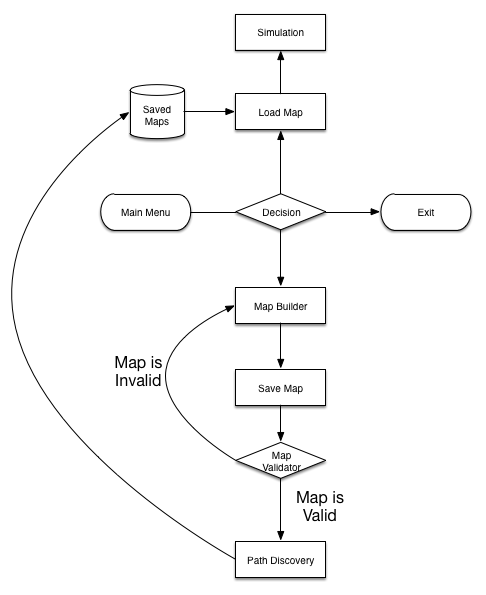
\includegraphics[width=4.5in]{activity_diagram}
\caption{Activity Diagram \label{fig:activitydiagram}}
\end{figure} 
 
\noindent The first window that appears on the screen consists of three basic buttons: Simulation, Map Builder and Exit. Once the user has pressed the map builder button will prompt to a new window where he/she will be able to build any kind of map from the available roads block on the side toolbar. Initially, the user will have to select if he/she wishes to create a new map or load an existing map from the user's file system of his/her own computer. Once the user has selected to create a new map, they must provide a name to the map and set grid width and height which is the place where they are going to add the road blocks. Then, the map builder view will be ready to use with all the functionalities displaying on the sidebars. After the user has done the desired design of the grid/map will be able to check if their map passes the validation. If the new map has not pass the validation process, the user will not be able to proceed with the simulation view. The correction of the invalid roads should be done and check again for validating the map. 
\newline

\noindent Filling in, the main idea behind simulation view is that the user will be able to load an existing map from the file system that has created before by using map builder as mentioned before. Although, the user has to select the desirable map from the existing list of the small pop-up window that appears. In the case where the user has selected a wrong map and wishes to open a new map it can simply select the Open button selection from the menu bar located on the top of the screen. All the valid maps that the user has generated on their personal computer, they are displayed on the list where the user can start the visual simulation. Once the user has selected the map the software adds traffic lights whenever it recognizes an intersection. The user is also able to manage the simulation of the map that he/she loads. The functionality of the speed scroll bar is to increase the motion of simulation from slow to fast or vice-versa. Then, the functionality of number of cars scroll bar manages the number of cars that can enter into the map grid. Once the user is sure about the map that he/she wishes to visualise the simulation, they are then able to use the available toolbar which includes the displayed timer, play, pause, stop, and refresh buttons. The buttons are there to manage both the timer and the simulation of the map; the timer is used to measure the time that the simulation holds (stopwatch functionalities). Obviously, the buttons accordingly can start the simulation, pause and stop the simulation, as well as manually update the timer using the step button.
\newpage

\section{Implementation}

\noindent In this section we will describe the software implementation and details about the simulator view as well as core functionalities like road editor block, path discovery. We will then discuss problem we had during the implementation of this core functionalities and how we have tried to solve them in order to have a reliable system and traffic simulator. In this section we might want to present some source code snipped in each of the specific section. We have to be clear on how we implemented each and why we think it was a good idea.
\newline

\noindent The software has a simple and intuitive frame page composed of two main screens. The first button is for the simulation view. The second one is for map builder view. First of all, when the user click on map builder view a pop up screen will appear on the user computer having three available options: create a new map, load a map or back to the main menu option. If the user click on create a new map he will be prompted to a small frame where the grid size must be specified. Once the user define the grid he want to use (e.g. 10x10) and assign a name on it the map builder screen will be executed. The screen present a grid on the centre of the page and a menu toolbar on the right side. The toolbar on the right side allow users to assembly road block based on their own preference and specifications. After the map has been assembled the user can save the map which will be then stored inside a folder so the user can import it later from the map builder menu. It is a crucial aspect to properly validate the proposed user map. This is way beyond the control of the user, the map validator function it is essential to allow the user to save and only run map that passed the validation process. As an example the code snipped below demonstrate how we detected this validation for a specific case such as a single intersection block. The simulation view panel will be used to run the actual traffic simulation according with the map that the user will use. Our system in fact allow the user to save different maps and store them for later use.

\subsection{Building Engine} 

In order to support the aforementioned components, such as agents, map builder, and simulation view, we needed to build an infrastructure. An engine that will build the required environment for these components. To begin with, we wrote the \textit{GridBuilder}, \textit{RoadBuilder}, \textit{AppDirBuilder}, \textit{ImagesBuilder} classes that gather and set the required information. The \textit{AppDirBuilder} class prepares all the directories needed in the file systems. Those are the folders in which we are going to be looking for the map related files. The paths that are chosen in order to create all the required directories, can be adjusted from the MainConfig configuration file, and in future implementation we could provide the user with the choice of the directory's location. \\

\noindent Moreover, the \textit{GridBuilder} class builds a grid of customizable size. Then, the \textit{RoadBuilder}, contains the roadGraphicsBuilder function, which takes a two dimensional array as an input, which represents the types of road blocks and locations in the grid (row and column number), so we can build the map. This array is retrieved by the following procedure. First, we access the TrafficInfrastructure file, which contains the names of all saved maps in our file system. By using the name of a map we can retrieve all the available Paths, as well as the BlockGraphicPoints, and the 2d array, which defines the location and type of the road blocks that will be used to construct the map. Finally, the \textit{ImagesBuilder} loads all of the images related to the road blocks that will be used to construct the map. Before the simulation starts when we open the simulation view. We preload all the images so that we can save cpu and memory and optimize the performance. The main reason is because of the repainting that is required from the Graphics class of Java in order to create the animation. In order to keep track of the location for all images used in our software, we created the GraphicsConfig configuration file. From that file, we can specify the graphics location, and, if necessary, change the images currently being used. This approach has allowed us to change the looks of our graphics two times. Our graphics development team has been making improvements until the very last moment and this configuration file made it less time consuming to us to make this alterations. Furthermore, in future implementations, we could allow our users to choose their own graphics (under predefined specifications that we would instruct), in order to personalize the look and feel of the simulation. 
\subsection{Map Builder} 
\noindent In order to make our software user friendly, we created an interface in which a user can create a grid with customizable size. This approach allowed us to build a simple map editor. So, using this grid, the user can create maps by placing road blocks on it. The editor enables users to view the different types of road blocks, choose whichever they want, and place it inside the grid in order to create a map and then validate it. In detail, when a user creates a map and chooses to save it, the MapValidator function is executed, which gets the newly created map's 2d array as an input. The array contains the information about the location and the type of the road blocks in the grid. If the map does not adhere to the rules an error is returned to the user. Each road block has to follow certain rules. Not all road blocks are compatible with each other. Using a switch statement, upon reading the type of block a series of checks is performed in order to ensure that it is valid. Additionally, during the validation, all starting and ending points are identified in order to assist the path discovery procedure that follows later. As an example of the validations that take place, a code snippet is presented below depicting the rules that have to be followed by the roundabout block:

\lstset{language=Java, framexleftmargin=10pt, framexrightmargin=10pt, frame=single, breaklines=true, }          % Set your language (you can change the language for each code-block optionally) 
\begin{lstlisting}[numbers=left, numberstyle=\small, numbersep=8pt,  framexleftmargin=1pt, framexrightmargin=10pt ] 

case RoadConfig.ROUND_ABOUT_BLOCK:{
	if((i<1 && j<1 && i+1<=map.length ) ||(map[i-1][j+1]!=RoadConfig.HORIZONTAL_BLOCK && map[i-1][j+1]!=RoadConfig.HORIZONTAL_ENTER_BLOCK) || (map[i+3][j+1]!=RoadConfig.HORIZONTAL_BLOCK && map[i+3][j+1]!=RoadConfig.HORIZONTAL_EXIT_BLOCK) || (map[i+1][j-1]!=RoadConfig.VERTICAL_BLOCK && map[i+1][j-1]!=RoadConfig.VERTICAL_ENTER_BLOCK) || (map[i+1][j+3]!=RoadConfig.VERTICAL_BLOCK && map[i+1][j+3]!=RoadConfig.VERTICAL_EXIT_BLOCK) || 
			(map[i-1][j]!=0 && map[i-1][j-1]!=0 && map[i][j-1]!=0 && map[i+3][j]!=0 && map[i+3][j-1]!=0 && map[i+2][j-1]!=0 && map[i+3][j+2]!=0 && map[i+3][j+3]!=0 && map[i+2][j+3]!=0 && map[i][j+3]!=0 && map[i-1][j+3]!=0 && map[i-1][j+2]!=0)){
		System.out.println("Round About Block failed Map Validations");
		return false;
	}
\end{lstlisting}

\noindent In this particular rule the roundabout, we make sure that all road ends of the roundabout are connected to vertical and horizontal single lane roads. Moreover, we make sure that any other blocks in the grid surrounding the roundabout are empty. If any of those rules fail, then a pop up is displayed to the user saying that "Map didn't pass validation and wasn't saved." In the future we would like to add more informative messages identifying exactly what was the error in the map that was created. 

\noindent After the validations have passed, as part of the save map process, the path discovery function executes as well. This is a recursive function that was inspired by the depth first search algorithm. It takes the newly created map's 2d array as an input and using this information it analyses the grid. Then, it creates another array in which it stores all the starting and ending points within the map. Depending on the block that was identified as a starting point, the function predicts the location of the next block, so if the starting point is a horizontal block, then the next block would be on the same row but next column of the grid. For each road block identified, a function getPath is called, which is different for every type of road block. This function returns the path points (in pixels) that are added in the overall path. If an intersection is detected, then a path is chosen, marked as visited, stored in the array containing the path, and then the path discovery function calls itself using that array as an input in order to find the rest of the possible paths from that intersection. The process that was just described occurs in order to identify all the possible paths from a specific starting point. However, since path points also have direction, this process is also performed for the ending points. So, all inverse paths are calculated as well. As a result, the information we needed to keep track of was increasing. For this reason, we created the RoadConfig configuration file, which included all of the block types, as well as all the possible directions so we can easily distinguish them from one another.

\subsection{Simulation View}
\noindent The simulation view class has been created and developed to allow the user to first create or load a set of predefined map or to simulate the traffic simulation of the saved and validated map. Generally, the main functionalities of the \textit{SimulationView} class are available to the user for managing the visual traffic simulation. The main idea of the simulation view is to allow the user to specify some characteristic of the simulation. We decided to offer three functionalities to the user that are available during the simulation. First, they can specify the number of cars used for the simulation, the second parameter allows users to set the speed of the overall simulation they want to run. The third parameter allows users to see and calculate the CO2 emission and the impact on the pollution level. Although behind the scenes, Java SWING commands have been used in order to have the visual representation of the entire GUI. First of all, the \textit{ApplicationFrame} is created in order to "host" all the other views that are part of the Graphical User Interface(GUI) and loads the content of them when they are called. In the \textit{SimulationView} class a Panel has created that holds \textit{JButtons, JLabels, Timer, JScrollPane} and the \textit{JMenuBar}. Each component has its own functionality (if necessary); such as JButtons calls ActionListeners for assigning some action when the user presses the button, though there is no need to create a function for a JLabel since it's a static component on the interface.\\

\noindent There are two menu bars in the simulation view: the first \textit{JMenuBar} consists of several \textit{JMenuItems} (such as File: New, Open, Main Menu, Exit, Edit). The second \textit{JMenuBar} consists of labels, buttons, and the timer. The values of \textit{Timer} are calculated in its own method where the appropriate estimations and checks (if-else-end statements) are happening for centiseconds, seconds and minutes. For visualising the timer, we have used the \textit{displayTimer.setText()}. Thus, we preferred to load images in the buttons, as well as all other graphics in our software through our ImageBuilder class which loads images from the Images folder of our software package. This only happens once, upon running our application, in order to save CPU and memory. The \textit{JButtons} that are used for manipulating the timer, and thus the simulation, are Play, Pause, Stop and Refresh. Each button individually has the referred \textit{ActionListener} which are listeners that assign events or actions to the corresponding button. For example: the listener of the Refresh button is used for resetting the timer and setting all the variables back to the defaults values which in our case is zero. 

\noindent In addition, we have created a \textit{JToolbar} which is located on the east side of the frame and it is the place where some functionalities are available to the user by using the \textit{JScrollpane} bars. The first \textit{JScrollpane} is used for the number of cars on the grid and it has a limitation of the minimum value to 1 and the maximum value to 100. The second \textit{JScrollpane} is a bar for representing the speed of the cars having the limitations from the value 1 to 10 which is slow and fast respectively. Thus, listeners have been settled accordingly to satisfy the scroll bars specifications. As an example, the code snippet below demonstrates the method implementing how we load an existing map that has passed its validation process to the simulation process and set the available functionalities to represent a map. 
\lstset{language=Java, framexleftmargin=10pt, framexrightmargin=10pt, frame=single, breaklines=true, }          % Set your language (you can change the language for each code-block optionally) 
\begin{lstlisting}[numbers=left, numberstyle=\small, numbersep=8pt,  framexleftmargin=1pt, framexrightmargin=10pt ] 

public void loadMap(String mapName){
		
		ArrayList<BlockGraphicPoint> arrBG =(ArrayList<BlockGraphicPoint>) FileRW.readObject(MainConfig.ROADBLOCK_PATH+"/"+mapName+MainConfig.ROADBLOCK_GRAPHICS_SUFFIX);
		GraphicsDrawer gDrawer = new GraphicsDrawer(50 ,mapName, arrBG , ib );
		playButton.addActionListener(new PlayListener(gDrawer));
		pauseButton.addActionListener(new PauseListener(gDrawer));
		stopButton.addActionListener(new StopListener(gDrawer));
		refreshButton.addActionListener(new RefreshListener());
		this.scrollPane = new JScrollPane(gDrawer);
		this.add(this.scrollPane);
		this.revalidate();
		this.validate();	}

\end{lstlisting}


\subsection{Agents} 

Our solution contains three different agents. As agents we define the \textit{StandardCar}, \textit{TrafficLight}, and \textit{RoadBlock} classes used in the simulation. All these agents are integrated into the simulation engine. Additionally, the road blocks are also integrated into the map editor and are also used by the map validator and the path discovery functions. To begin with, cars have a specific position, which is defined by X and Y coordinates of continuous space, in pixels. However, in order to identify their position in the grid, we have to divide their coordinates by the block size, which corresponds to the size of a cell in the grid. 

\begin{lstlisting}[numbers=left, numberstyle=\small, numbersep=8pt,  framexleftmargin=1pt, framexrightmargin=10pt ] 

gridX = this.carX/GraphicsConfig.BLOCK_SIDE_SIZE;
gridY = this.carY/GraphicsConfig.BLOCK_SIDE_SIZE;

\end{lstlisting}

\noindent Moreover, the cars are assigned a path, a direction, rotation angle, and driver type, which defines their speed, acceleration, and deceleration and a car type, which defines its CO2 emission. In order to keep track of the car's progress in the path, it contains a counter. In order to mitigate the issue of the car's interaction with other cars, we included two security distance attributes in the \textit{Car} class. The first one, is called securityDistance, and changes in relation to the speed of the car to ensure that a certain distance is kept between two cars that are moving. There is also the securityZeroDistance, which is used to define the distance between two cars that are stopped. Whenever a car is in a double lane road, in order to support multiple line usage, we had to include lane choice values, which would notify the cars about the lane they should be on, as well as getting information about the location of other cars around them. Furthermore, we implemented a function that defines if car can change lanes. While testing, we found that acceleration in the form of incrementing the speed by one for every timer cycle, does not represent a realistic scenario. In order to provide cars with a smooth acceleration, we related the speed, which is defined in pixels per second, with a constant values that represents the acceleration that depends on the driver's behaviour. This way by keeping this constant value we limit the speed increments to gradually increase the speed and accomplish a smoother animation of the car's acceleration. The function updateSpeed calls the acceleration and deceleration functions, in order to provide realtime changes in the speed of the cars during the simulation. 


\begin{lstlisting}[numbers=left, numberstyle=\small, numbersep=8pt,  framexleftmargin=1pt, framexrightmargin=10pt ] 

public void acceleration(){
	if (((RoadBlock)this.roadBlock[this.carX/GraphicsConfig.BLOCK_SIDE_SIZE][this.carY/GraphicsConfig.BLOCK_SIDE_SIZE]).getSpeedLimit()>this.speed){
this.accelerationCounter+= this.acceleration;
if (accelerationCounter>1){

	this.speed++;
	this.accelerationCounter-=1;
}
	}
}
\end{lstlisting}

\noindent On the other hand, the deceleration of the car is related to the final speed that needs to be reached by the car, and the distance in which it needs to reach that speed. 

\begin{lstlisting}[numbers=left, numberstyle=\small, numbersep=8pt,  framexleftmargin=1pt, framexrightmargin=10pt ] 
public void deceleration(int distance, int finalDeceleration){
	double decelerator = ((double)speed - finalDeceleration)/(double)distance;
	this.decelerationCounter+= decelerator;
	if(this.speed>this.decelerationCounter){
	if(decelerationCounter>=1){
speed-=decelerationCounter;
decelerationCounter-=(int)decelerationCounter;
	}
} else {
	speed = 0;
}
}
\end{lstlisting}

\noindent Both\textit{Car} and \textit{TrafficLight} classes, contain a draw function, which identifies the type of block they agents are placed on, in the grid, and the direction, in order to be represented either vertically or horizontally. \\

\noindent Traffic lights also have the same X and Y coordinate scheme as the car. Additionally, in order to distinguish the traffic lights that are placed on the first or second of the two lane roads, we included a type attribute as well as a trafficLightState attribute which defined if the traffic light is green, yellow, or red. For this reason, our simulationBuilder contains three different classes that manage traffic lights depending on the type of intersection: \textit{TrafficLightSetDoubleIntersection}, \textit{TrafficLightSetMixedIntersection}, \textit{TrafficLightSetSigleIntersection}. Additionally, the traffic light location depends on the direction of the path. 
Finally, the \textit{TrafficLightsBuilder} class analyzes the grid and finds all intersections in order to define the positions of the traffic lights. Then, the traffic light is placed in an array, which is used as an input in order to reprint the traffic lights on the map during the simulation. Depending on the type of intersection, the traffic lights are also placed on another array, which is used for the traffic light management from the three classes mentioned earlier. \\

\noindent Agents are dynamic during simulation. The road blocks are defined as agents too because during the simulation a road block could be empty, or not and it could also have traffic lights on it. As mentioned before, road blocks have a predefined speed limit depending on their type. Finally, they also have access to the array that stored all the cars in the map, as well as all the traffic lights. 
\newpage

\section{Team Work}

\subsection{Team Management} Team work and smooth communication between members have been a key point for the successful development of the project. During our activity as a group we have to overcome different problems and tried to minimize discussion. Stuck in traffic used the expertise of each member in all the different cycle phases of the project in order to complete all the required task efficiently. Our initial goal was to work together as a team, understanding the project specifications and implementing software that can be used for future development. This approach geared us into the correct manner for better cooperation and understanding of different team work skills and values. The project requirements were met before the deadline, allowing the group to reflect on our decisions and implementations. If we consider the software requirements and the tasks of the individual, we have concluded that the tasks have been successfully achieved our and main objectives are completed. \newline

\noindent The solution we designed provide the users with a list of maps from which they can choose one to perform their simulation, as well as customizing the number of cars, and other parameters. In order to deliver this task in the best way possible we aimed to provide users with a good quality User Experience Design (UEX). As a result of this, the group has been split into two teams. One team was working on the main system development and the other team was in charge of designing and developing the user interface. Specifying the requirements that have been implemented later such as; the functionality of increasing and decreasing the number of cars and specifying the simulation speed. The initial split of the team created a small problem because the work was not properly synchronized and organized though after some clarifications we all agreed a proper way of how to proceed. For this reason we also created the separated branch in the Github only dedicated to the GUI implementation. Even though all members will actively participating during all phases of the project development we have defined the specialization of each member:

\begin{itemize}

\item Project coordinator: Filippos Raditsas. \item Analysis: Filippo Mariani. \item Software Design/Development: Maxim Vasilishin. \item Graphics: Maximimilian Nikolaidis. \item GUI Design \& Development: Antria Dimitriou, Filippo Mariani. \item QA: Antria Dimitriou.

\end{itemize}

\noindent The project coordinator's responsibility was mainly to ensure that all the group member respect their given deadlines for the assigned task and to assist in the interpretation of the requirements between the lead developer and the rest of the members. He was also in charge of defining all team meetings and activities assigned during the different week of the project. The analysis process helped us understand which technologies, programming languages, solutions, and approaches to follow to determine the best route for a successful implementation. We discussed this with different point of view taking in consideration the main requirement involved with the implementation and possible problem related to its complexity and time frame. After actively discuss the analysis of the project we then move straight to the software design and implementation phase. Following the analysis specification we come up with an high level design and description of the software and its requirements. We followed the spiral model that allow us to divide the project deliverables in small cycle and visible tasks for the given phase. Part of the requirements of this project was to develop everything from scratch where possible. For this reason our graphics has been designed entirely from scratch without using any third-party library or any external resource. We designed all the agents deployed in our software, all the buttons and all the different kind of road block. Photoshop was used to develop all the graphics and we also had to apply light changes to the different images in order to adapt it properly for our software. All of the above activity were part of the requirement in order to have a reliable software and a clear way forward for the plan. Nevertheless Quality Assurance it has been one of the main activity that involved us during the project. During every cycle we have to test our software and our implementation technique. This procedure allow us to fix potential bug before it was too late and also helped us in order to understand which part of the software needed more attention and optimizations.

\subsection{Methodology}

\noindent The Spiral model, has been used in order to keep up to date with completing the project. As defined in \cite{boehm2000spiral} "Spiral development is a family of software development processes characterised by repeatedly iterating a set of elemental development processes and managing risk so it is actively being reduced". The spiral model is a risk driven process that allows all areas of the spiral to be created simultaneously in order for quick delivery. The spiral model is more appropriate for this kind of project, as it will help us mitigate risks such as steep learning curve during the development phase, limited time, and individual member's unforeseen circumstances and enable us to add features and ideas to the project. We have divided the spiral model in 4 main phases, Requirements Analysis, Risk Analysis, Development and Evaluation. During the requirements analysis, upon testing and evaluating existing solutions we decided to create our own simulation engine and defined the requirements based on the time constraints given on each spiral cycle. Each spiral cycle involved risk evaluation, in detail we split the tasks and set the requirements of each cycle depending on the members availability and technical knowledge. The development phase of each cycle involved assigning tasks to the corresponding members. Finally, each spiral cycle involved evaluation including regression testing and verification that the requirements were met. 

\begin{figure}[h] 
\centering 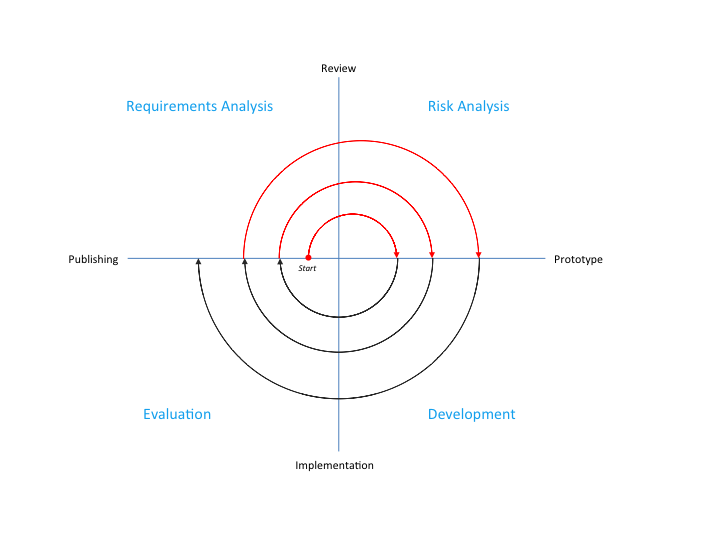
\includegraphics[width=4.5in]{spiral} 
\caption{Spiral Model} 
\end{figure}
\newpage

\noindent Effective and in time communication between partners has been a key point for having a proper project development. We have agreed to have a full group meeting every Wednesday at 17:00 in the MSc lab 534 to discuss any issues that raised during the weekly tasks. There were also informal meeting that took place between the available members during the week in order to discuss minor changes and alterations. Informal meetings were not mandatory for all members to attend. They took place mainly to accommodate individual needs and responsibilities, such as work, timetabling collusions with lectures, other coursework, etc. Github was another valuable resources that helps us during the project to maintain a proper team work contribution in a very organized way. Our Github "Stuck In Traffic" repository can be accessed at the following link: \url{https://github.com/philiprad/}stuckintraffic. Github was used to upload development progress online and to allow members to maintain an up to date software development environment.

\noindent For internal communication that does not take place in person, the team have set up two mediums of communication;

\begin{itemize} \item Slack Framework: https://slack.com/ We have created a group account to communicate and exchange files
\item Skype: http://www.skype.com/en/ We have created an internal schedule for online meetings. \end{itemize} \newpage

\subsection{Project Scheduling}

\noindent In order to maintain a proper time management we have created and followed a gantt chart. The chart has been used in order to set a proper structure for internal project deliverables and to have a more accurate and reasonable workflow distribution among our group during the project time. We have divided the project in two different gantt charts depicting two different periods, one for the intermediate project deadline as shown in Figure \ref{fig:ganttChartOld}, and the second one for the final project deadline as shown in Figure \ref{fig:ganttChartNew} .

\begin{figure}[h] 
\centering 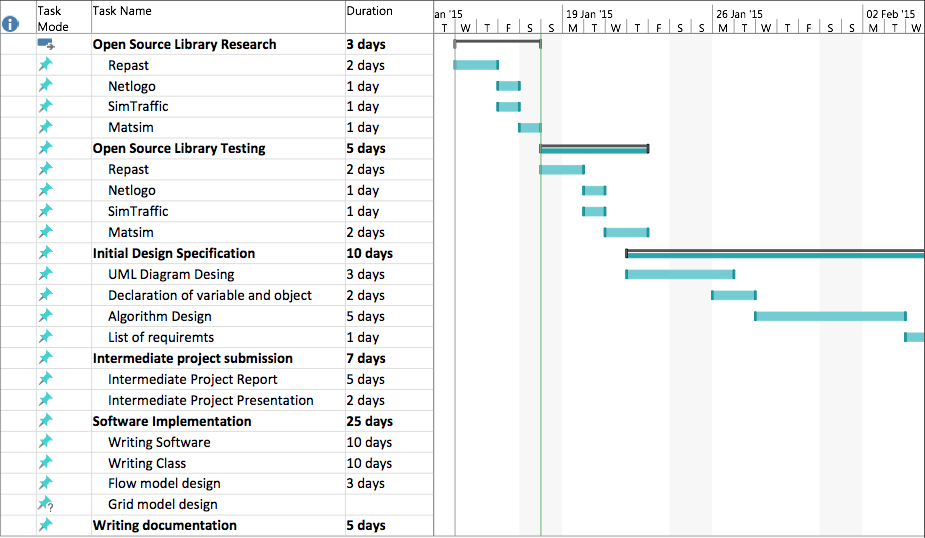
\includegraphics[width=6in]{ganttchart_old} 
\caption{Gantt Chart depicting main tasks and timetable for intermediate report \label{fig:ganttChartOld}} 
\end{figure}
\newpage
 
\begin{figure}[h2] 
\centering 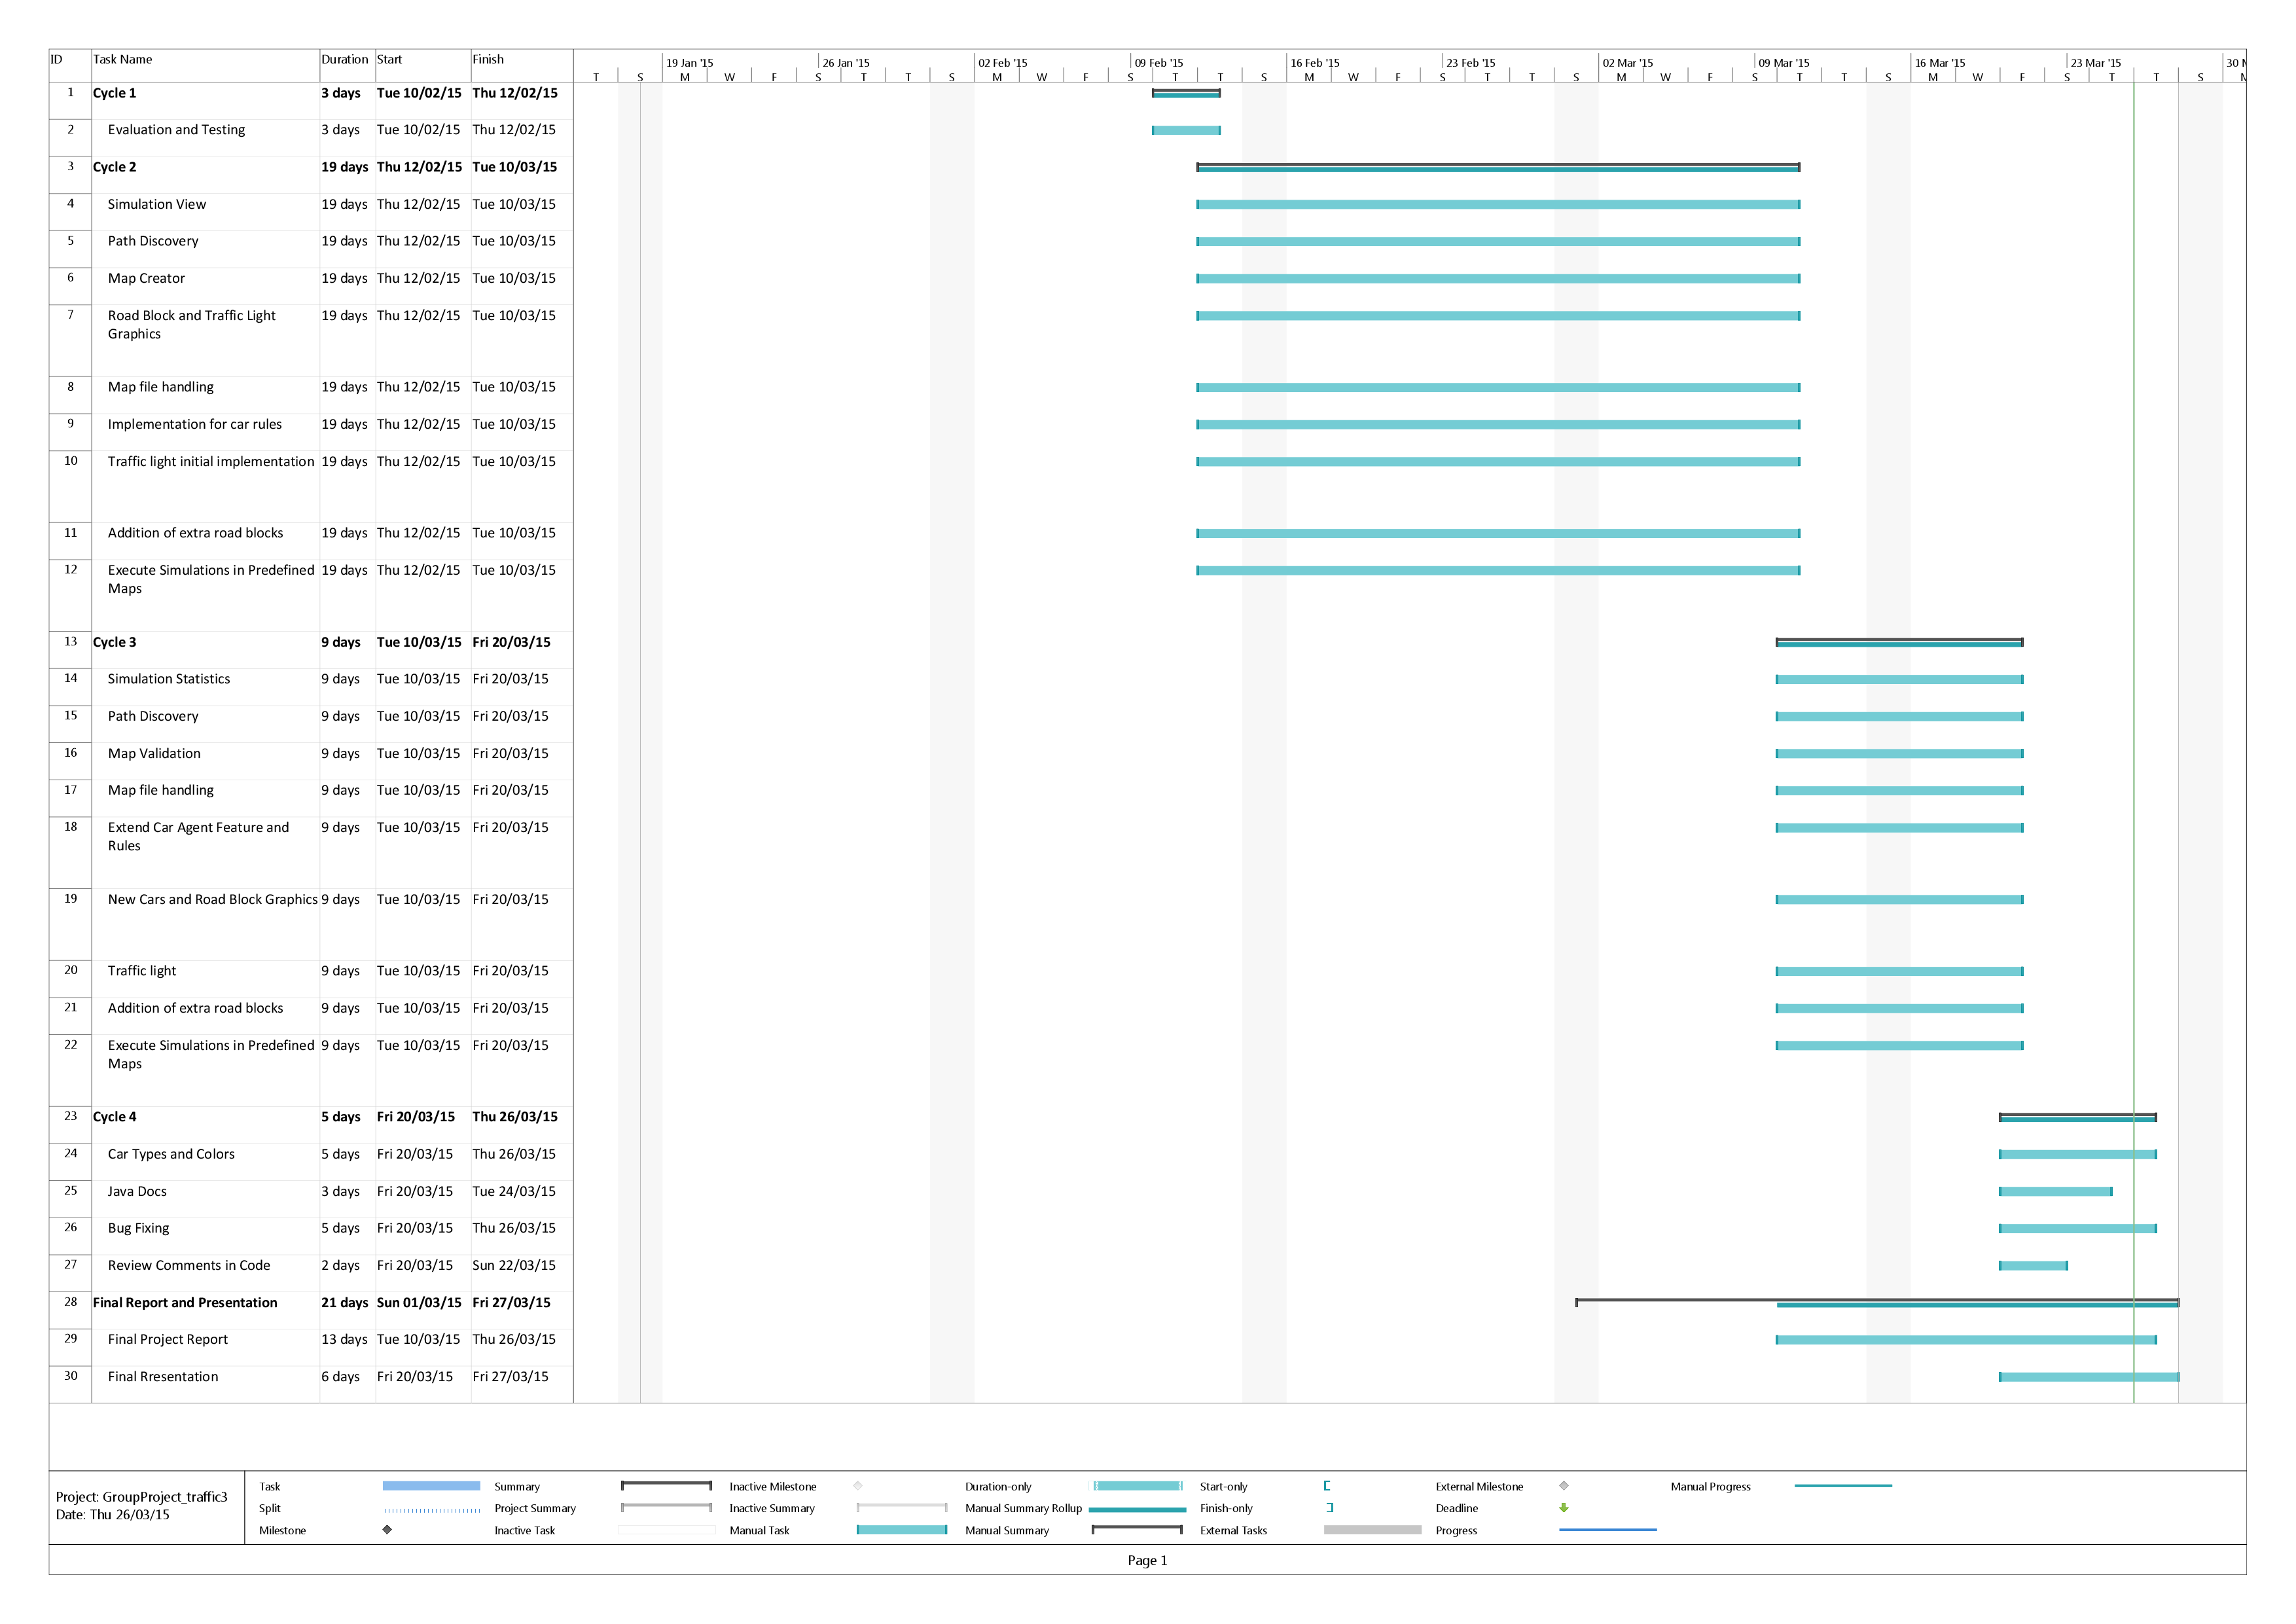
\includegraphics[width=6in]{gantt_chart}
\caption{Gantt Chart depicting main tasks and timetable for final software and report submission \label{fig:ganttChartNew}} \end{figure}
\newpage


\section{Project Evaluation}

\noindent During the project we came across different problems and issues mainly related to the software implementation and the design phase. First of all, in the beginning our goals were very ambitious and unrealistic. Furthermore, by the time we managed to set a realistic and reasonable scope, each one of us had different approaches and ideas in mind. When we concluded on the idea we actually developed, the main problem was the technical gap of our team members with the lead developer. Furthermore, the lead developer was responsible for building the engine upon which the agents, the map builder and the GUI would be developed. Thus, the software was designed in a way that one did not need to fully understand all the software components in order to start working on their tasks. Whenever it was need, our coordinator was responsible for the interpretation of technical requirements into business requirements and vice versa.\\

\noindent Most of our team members were not confident when using Github and this caused us many problems during the development. Even though we initially intended to use pull requests, after experimenting with Github we decided to create different branches of our master Github repository in order to keep working at the same time on different task without affecting the master branch files. For example, the Filippo\_Andria branch (\url{https://github.com/philiprad/stuckintraffic/tree/Filippo_Andria}) has been created only for the GUI design and implementation. By doing so, we allowed our lead developer to evaluate the proposed work, provide feedback for the proposed version of the GUI, and finally reintegrate whichever parts of the branch needed to be transferred to the original. 
\newline

\noindent At the beginning we had to split each task properly given the knowledge of the people in the group. As we started everything from scratch, we had many different tasks, such as graphics, getting familiar with GUI development using Java Swing, memory management and overall performance, smooth animation, an efficient and user friendly map builder, and most importantly time management. The main problem we faced is that the main engine took much longer than expected to be completed. As a result, although we have a concrete and powerful engine, we didn't have time to implement many features to fully utilize its capabilities. For example, we didn't have the time to provide a panel that allows users to choose their own graphics for the roads or the cars by exposing the aforementioned corresponding configuration files. Additionally, we didn't provide a very detailed report regarding statistical information of the simulation. Finally, in the simulation, we didn't add the option to have traffic signs instead of traffic lights, parking spots, emergency lane support, and pedestrians crossing the road. All these features that were not implemented could show the full potential of our software.\\

\noindent Even though our major weakness is the fact that we have not utilized our engine's full potential, this is one of our strongest points at the same time. We have achieved to build a fully extensible engine, upon which developers could implement their ideas. It can be altered to support other types of simulations. As long as new agents and graphics are added, our simulation engine can be easily adapted for different types of traffic, such as vehicle traffic in an airport or any other scenario, or even a simple video game, e.g. sims city. We developed our system is a way that will easily allow developers to customize and improve our functionalities and users to make use of our software's full potential. After completing this task we have encountered some other problems mainly related to the map validation in the simulation view, which were mainly addressed by systematic regression testing. During this phase we have to make a lot of test for the block validation in order to avoid validating non usable map. \\

\noindent Given our current software structure and class division we believe that the above functionalities will be implemented easily in future version of the "Stuck in Traffic Simulator". Another important future work implementation is the aim of adding some statistical report generator about current traffic simulations such as allow the user to obtain information about number of cars, average car speed or define weather condition. Another future implementation we propose for our system is the support for emergency vehicle and how the traffic flow will change according with their presence. Finally, an immediate next step for our software is to complete the interaction of the cars in the roundabout. So far collisions are not avoided and distances are not always kept. The roundabout is one of the tasks that we predicted that we have had completed, but unfortunately due to the bugs that were discovered we did not have time to finish it.
\newline

\noindent However, not all the problems we had were related to technical issue. Another problem is that one of our group member was away for 10 days during the project. This was a problem for us because we had to split all the workload between the rest of us. In fact, this is one of the reasons we decided to adopt the spiral model, which allowed us to help each other during different project phase. In the last week of the project, we kept finding new bugs, and rule collisions in the simulation. In fact, our software has many bugs relating to the simulation and the car interaction. Fortunately, the major bugs, which were mostly related to keeping safe distances between the cars, as well as making the cars respect both each other and the traffic rules were solved and ended up having a stable and presentable version of the software. However, there are certain scenarios that still have bugs. In some cases, bugs, such as a deadlock on major traffic jams, unintentionally provide us with interesting scenarios and features that we originally did not think we would have time to implement. As the project moved along we came up with new ideas and aspirations that unfortunately were automatically discarded as new bugs kept being discovered and whose fixing was considered a top priority of our development progress.
\newpage

\section{Peer Assessment}

\noindent 
The peer assessment takes place to ensure a fair distribution of points for each member upon completion of the project. The amount of points awarded to a particular member may alter based on their contribution to the project and amount of work they put towards helping other members. Since there are five members in the team and there are 100 points to give accordingly the ultimate goal of our team is to evenly distribute the points assuming that we will all contribute the same amount of work and will collaborate smoothly and efficiently. The criteria that have been taken into account for each members is the participation, how much work has been submitted by each member, member\ 's enthusiasm and general involvement with the project activity.
\newline

\noindent The way in which a member will be allocated points is by the following table, each member will be able to give out one hundred (100) points in total. The points can range from 0 to 100 inclusive, also the members are able to assign decimal points to members, but the total amount of points must equal one hundred (100).


\begin{table}[h]
\resizebox{\textwidth}{!}{%
\begin{tabular}{|l|l|l|l|l|l|}
\hline
Name                  & Filippo Mariani & Maxim Vasilishin & Filippos Raditsas & Maximilian Nikolaides & Antria Dimitriou \\ \hline
Filippo Mariani       & -               & 25               & 25                & 25                    & 25               \\ \hline
Maxim Vasilishin      & 25              & -                & 25                & 25                    & 25               \\ \hline
Filippos Raditsas     & 25              & 25               & -                 & 25                    & 25               \\ \hline
Maximilian Nikolaides & 25              & 25               & 25                & -                     & 25               \\ \hline
Antria Dimitriou      & 25              & 25               & 25                & 25                    & -                \\ \hline

\end{tabular}
}
\caption{Peer Assessment table}
\end{table}
%\clearpage


%\addtocontents{toc}{\vspace{2em}} % Add a gap in the Contents, for aesthetics
%\backmatter
\newpage
\bibliographystyle{ieeetr}
\bibliography{related_work}

\newpage
\section*{QA Testing Appendix} % Main appendix title


\begin{figure}[h2] 
\centering \includegraphics[width=6in]{QA_TestCases}
\caption{Table depicting test cases for the map creator} 
\end{figure}

\newpage
\section*{GUI Screenshots} % Main appendix title


\begin{figure}[h2] 
\centering 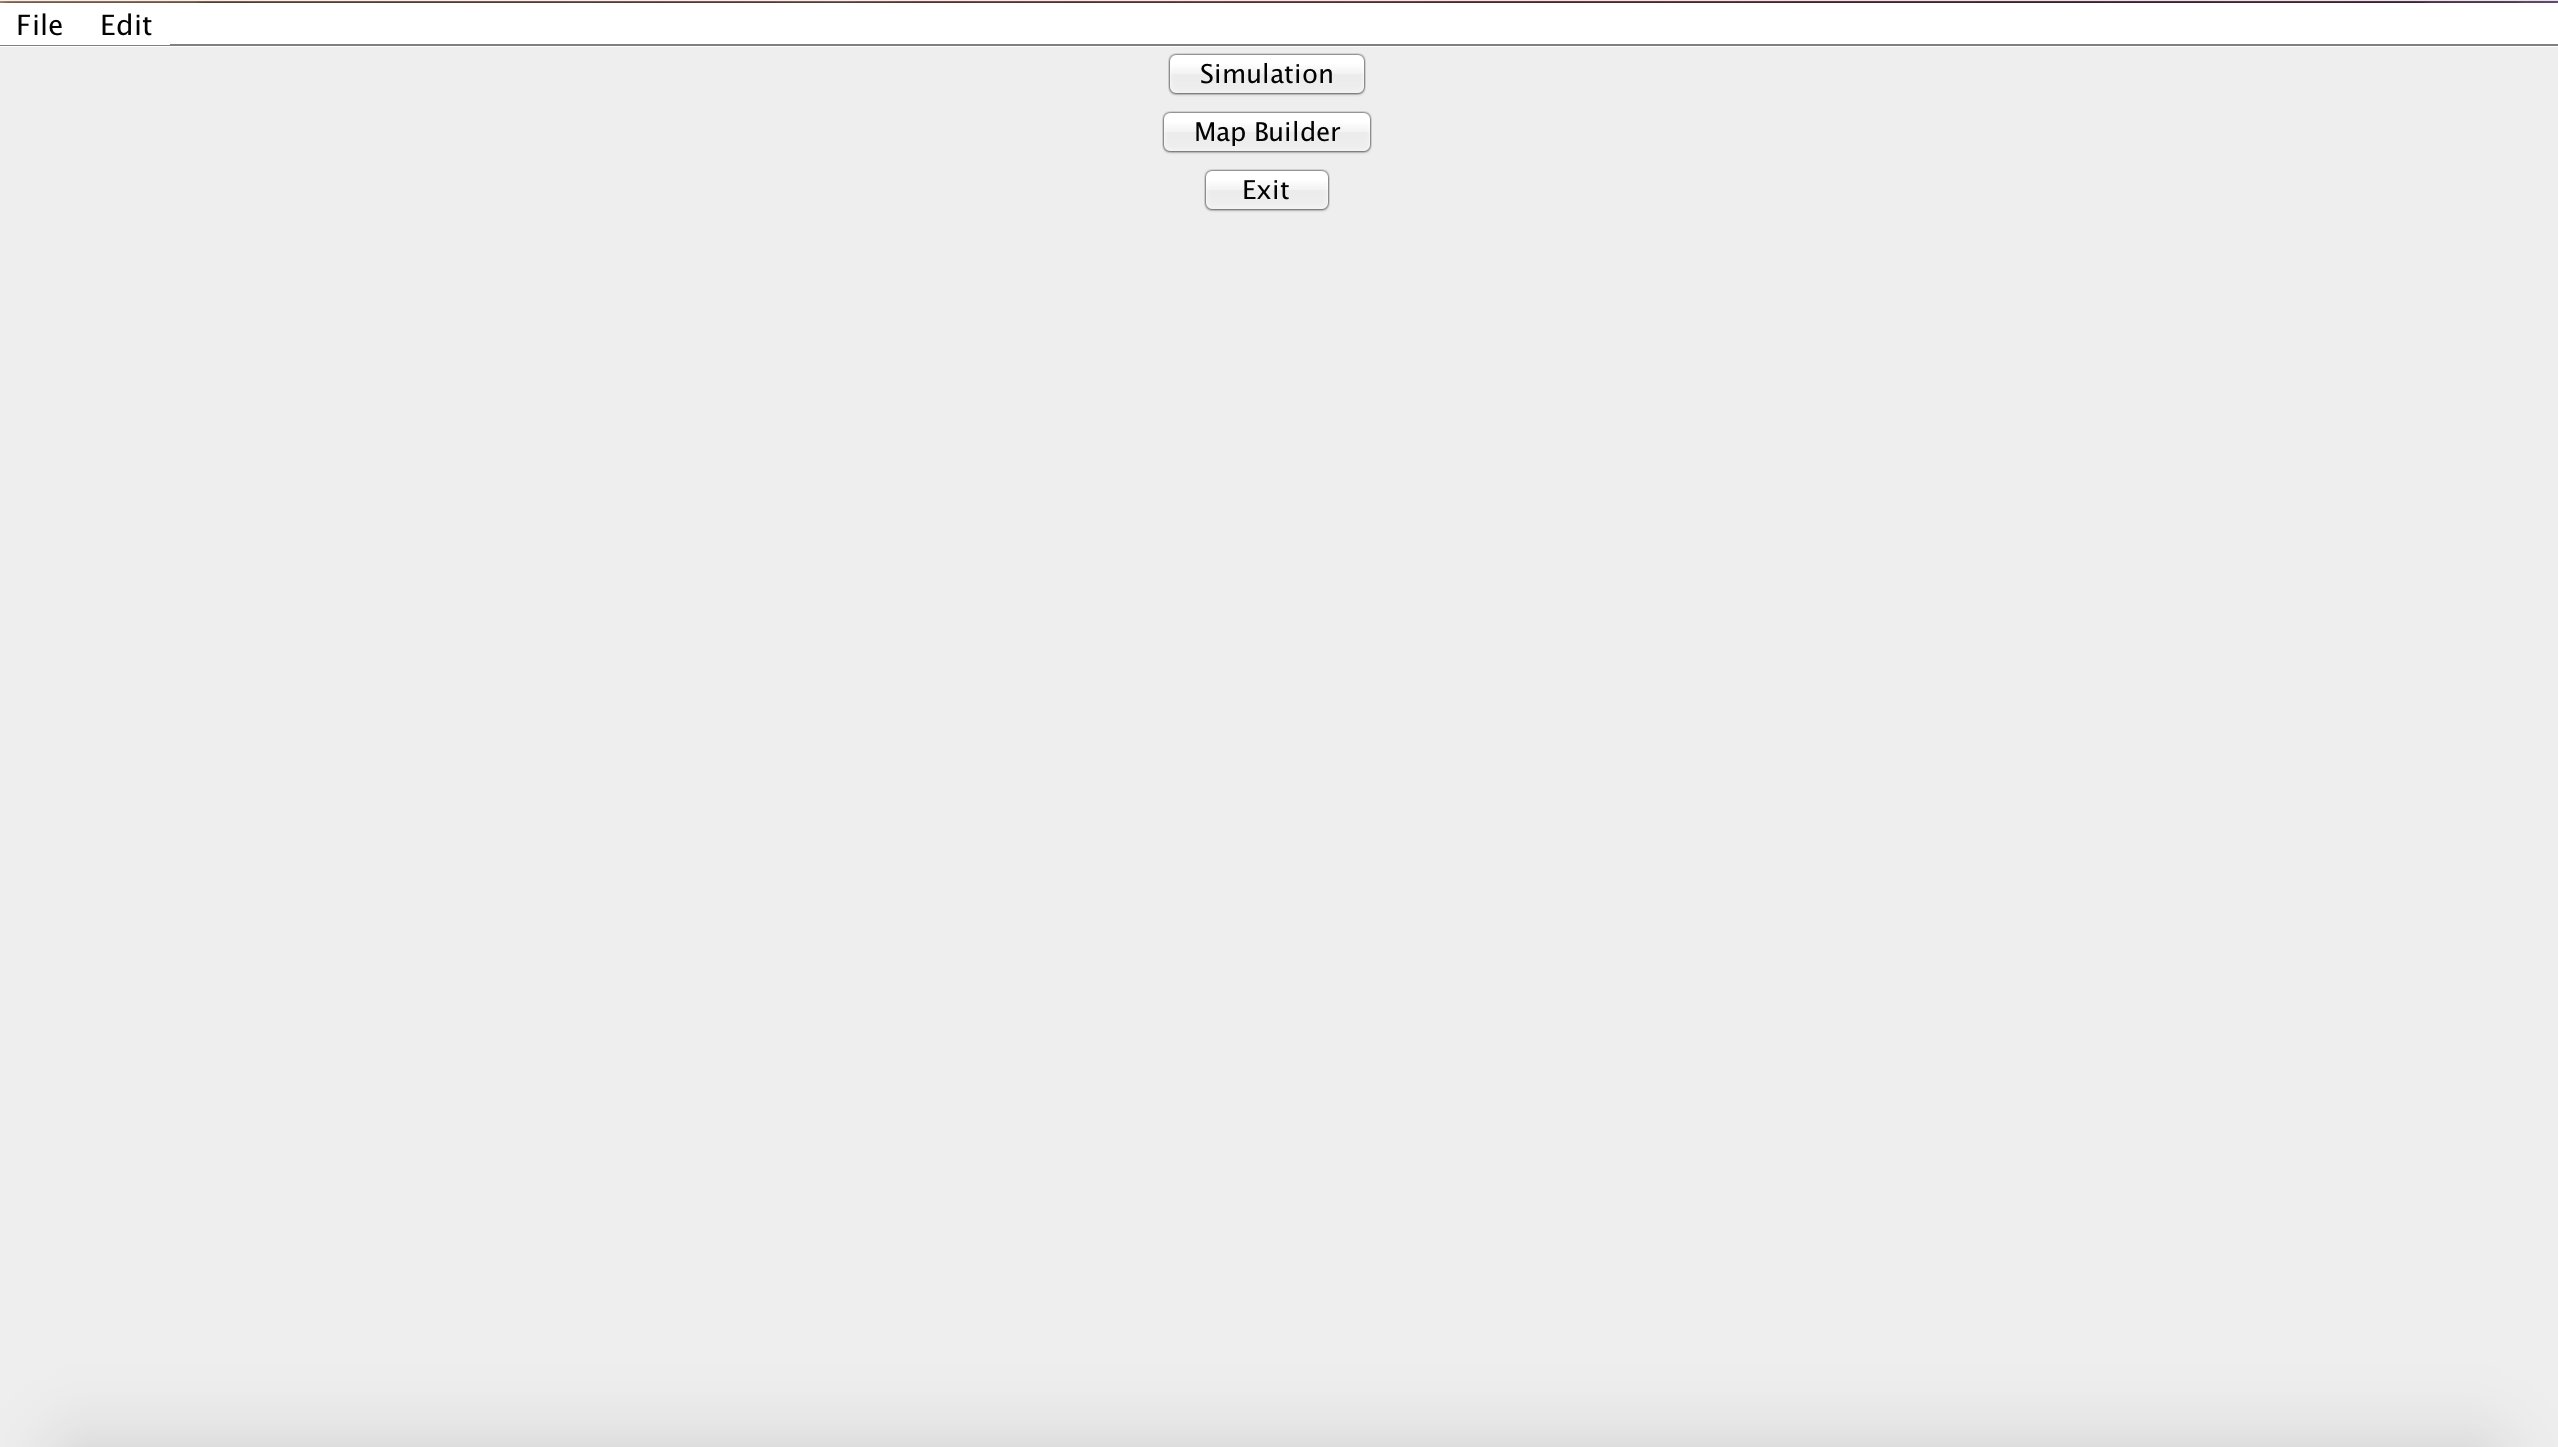
\includegraphics[width=6in]{img1}
\caption{Main Menu} 
\end{figure}

\begin{figure}[h2] 
\centering 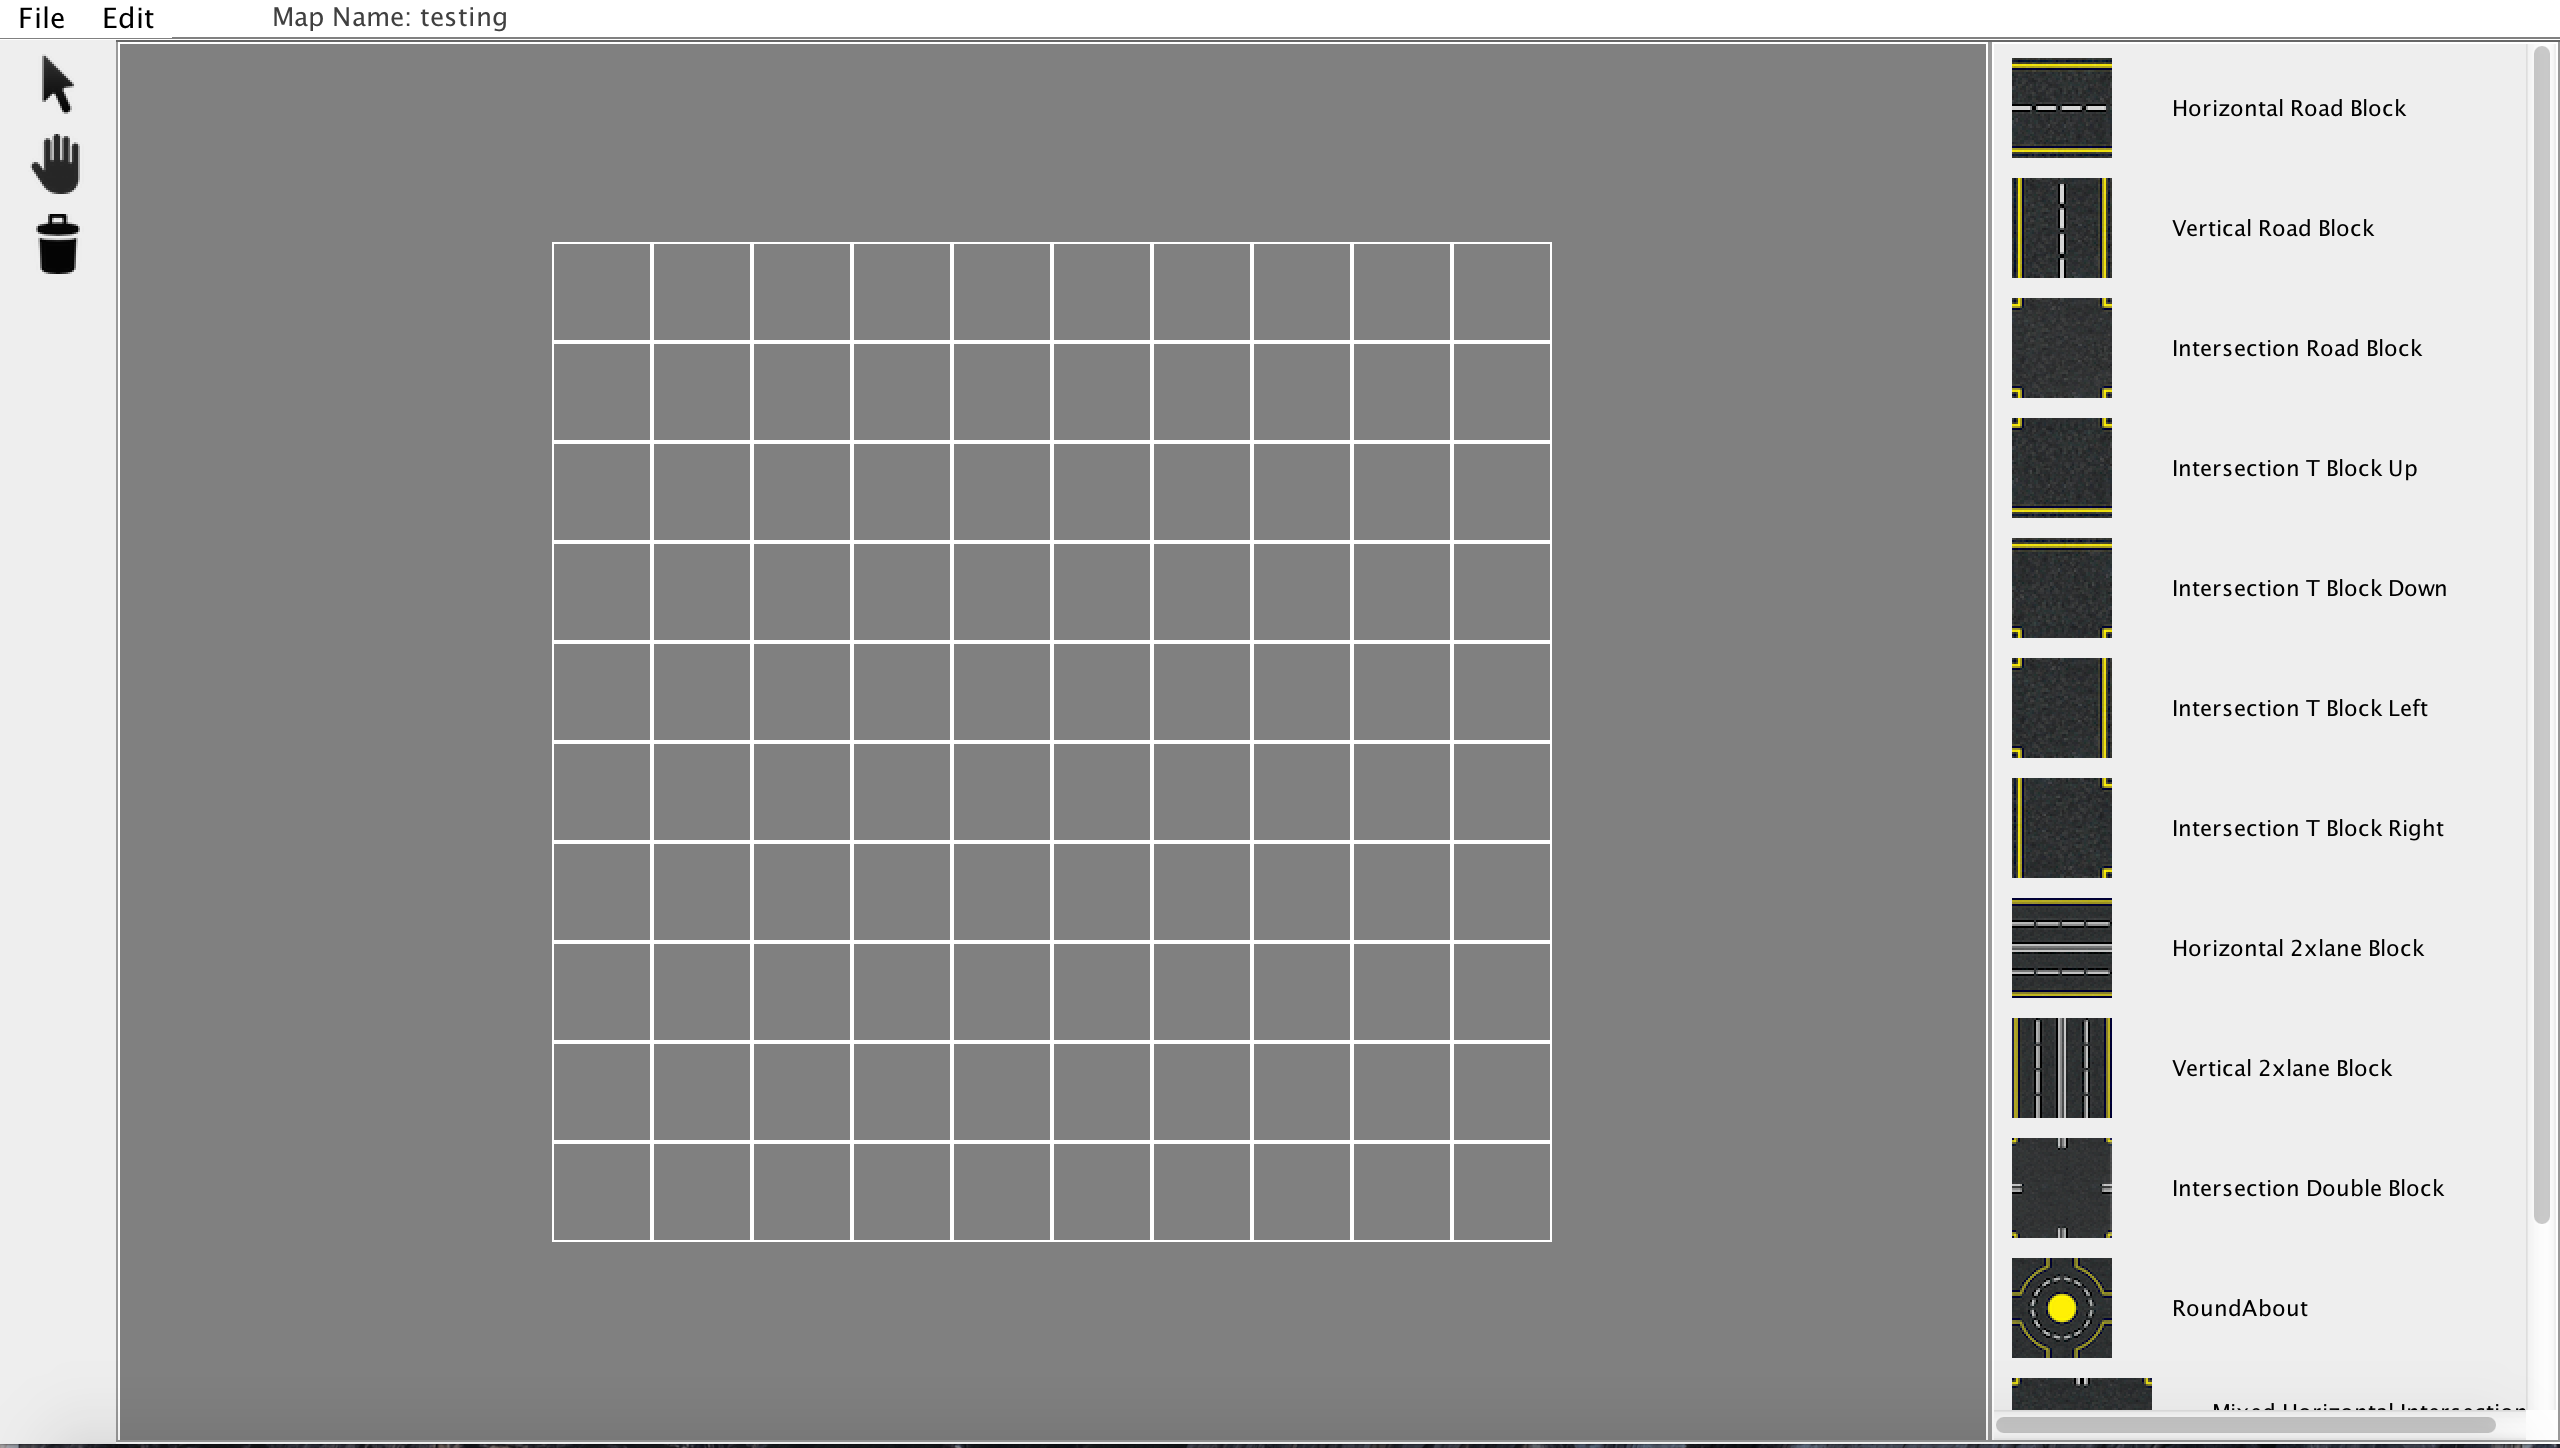
\includegraphics[width=6in]{img2}
\caption{Map Builder (Initial Page)} 
\end{figure}

\begin{figure}[h2] 
\centering 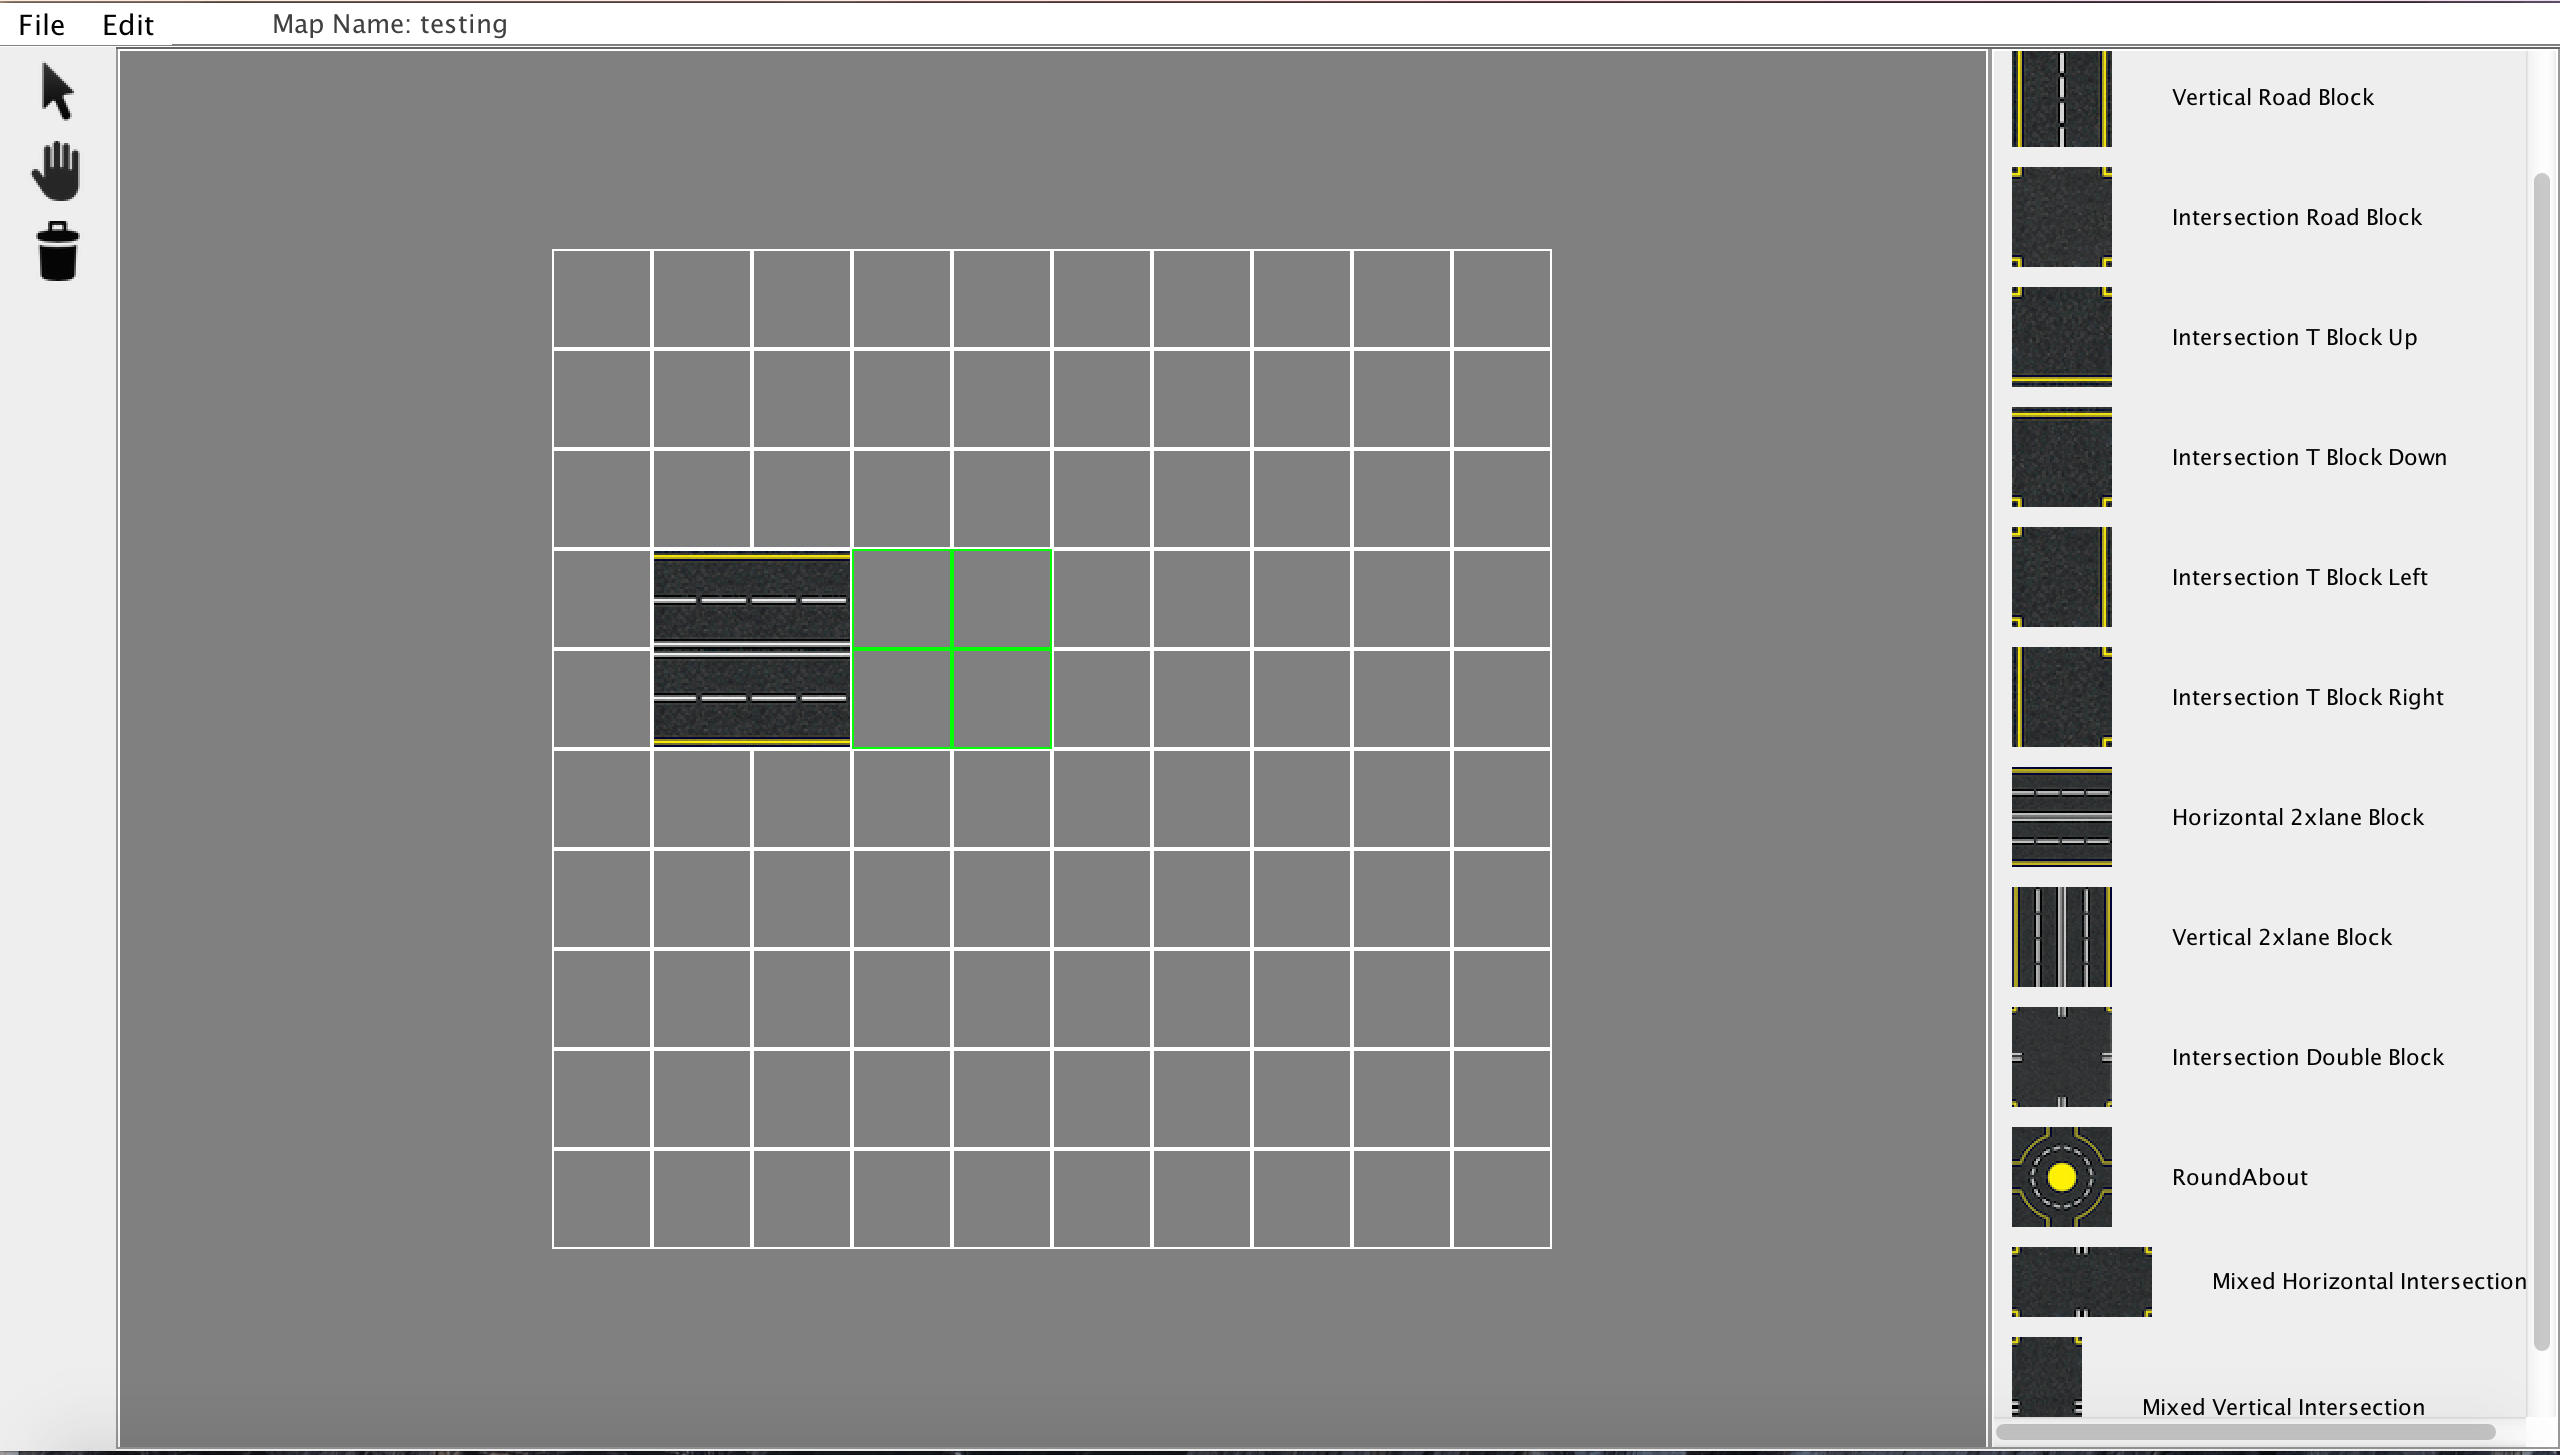
\includegraphics[width=6in]{img3}
\caption{Map Builder with one block} 
\end{figure}

\begin{figure}[h2] 
\centering 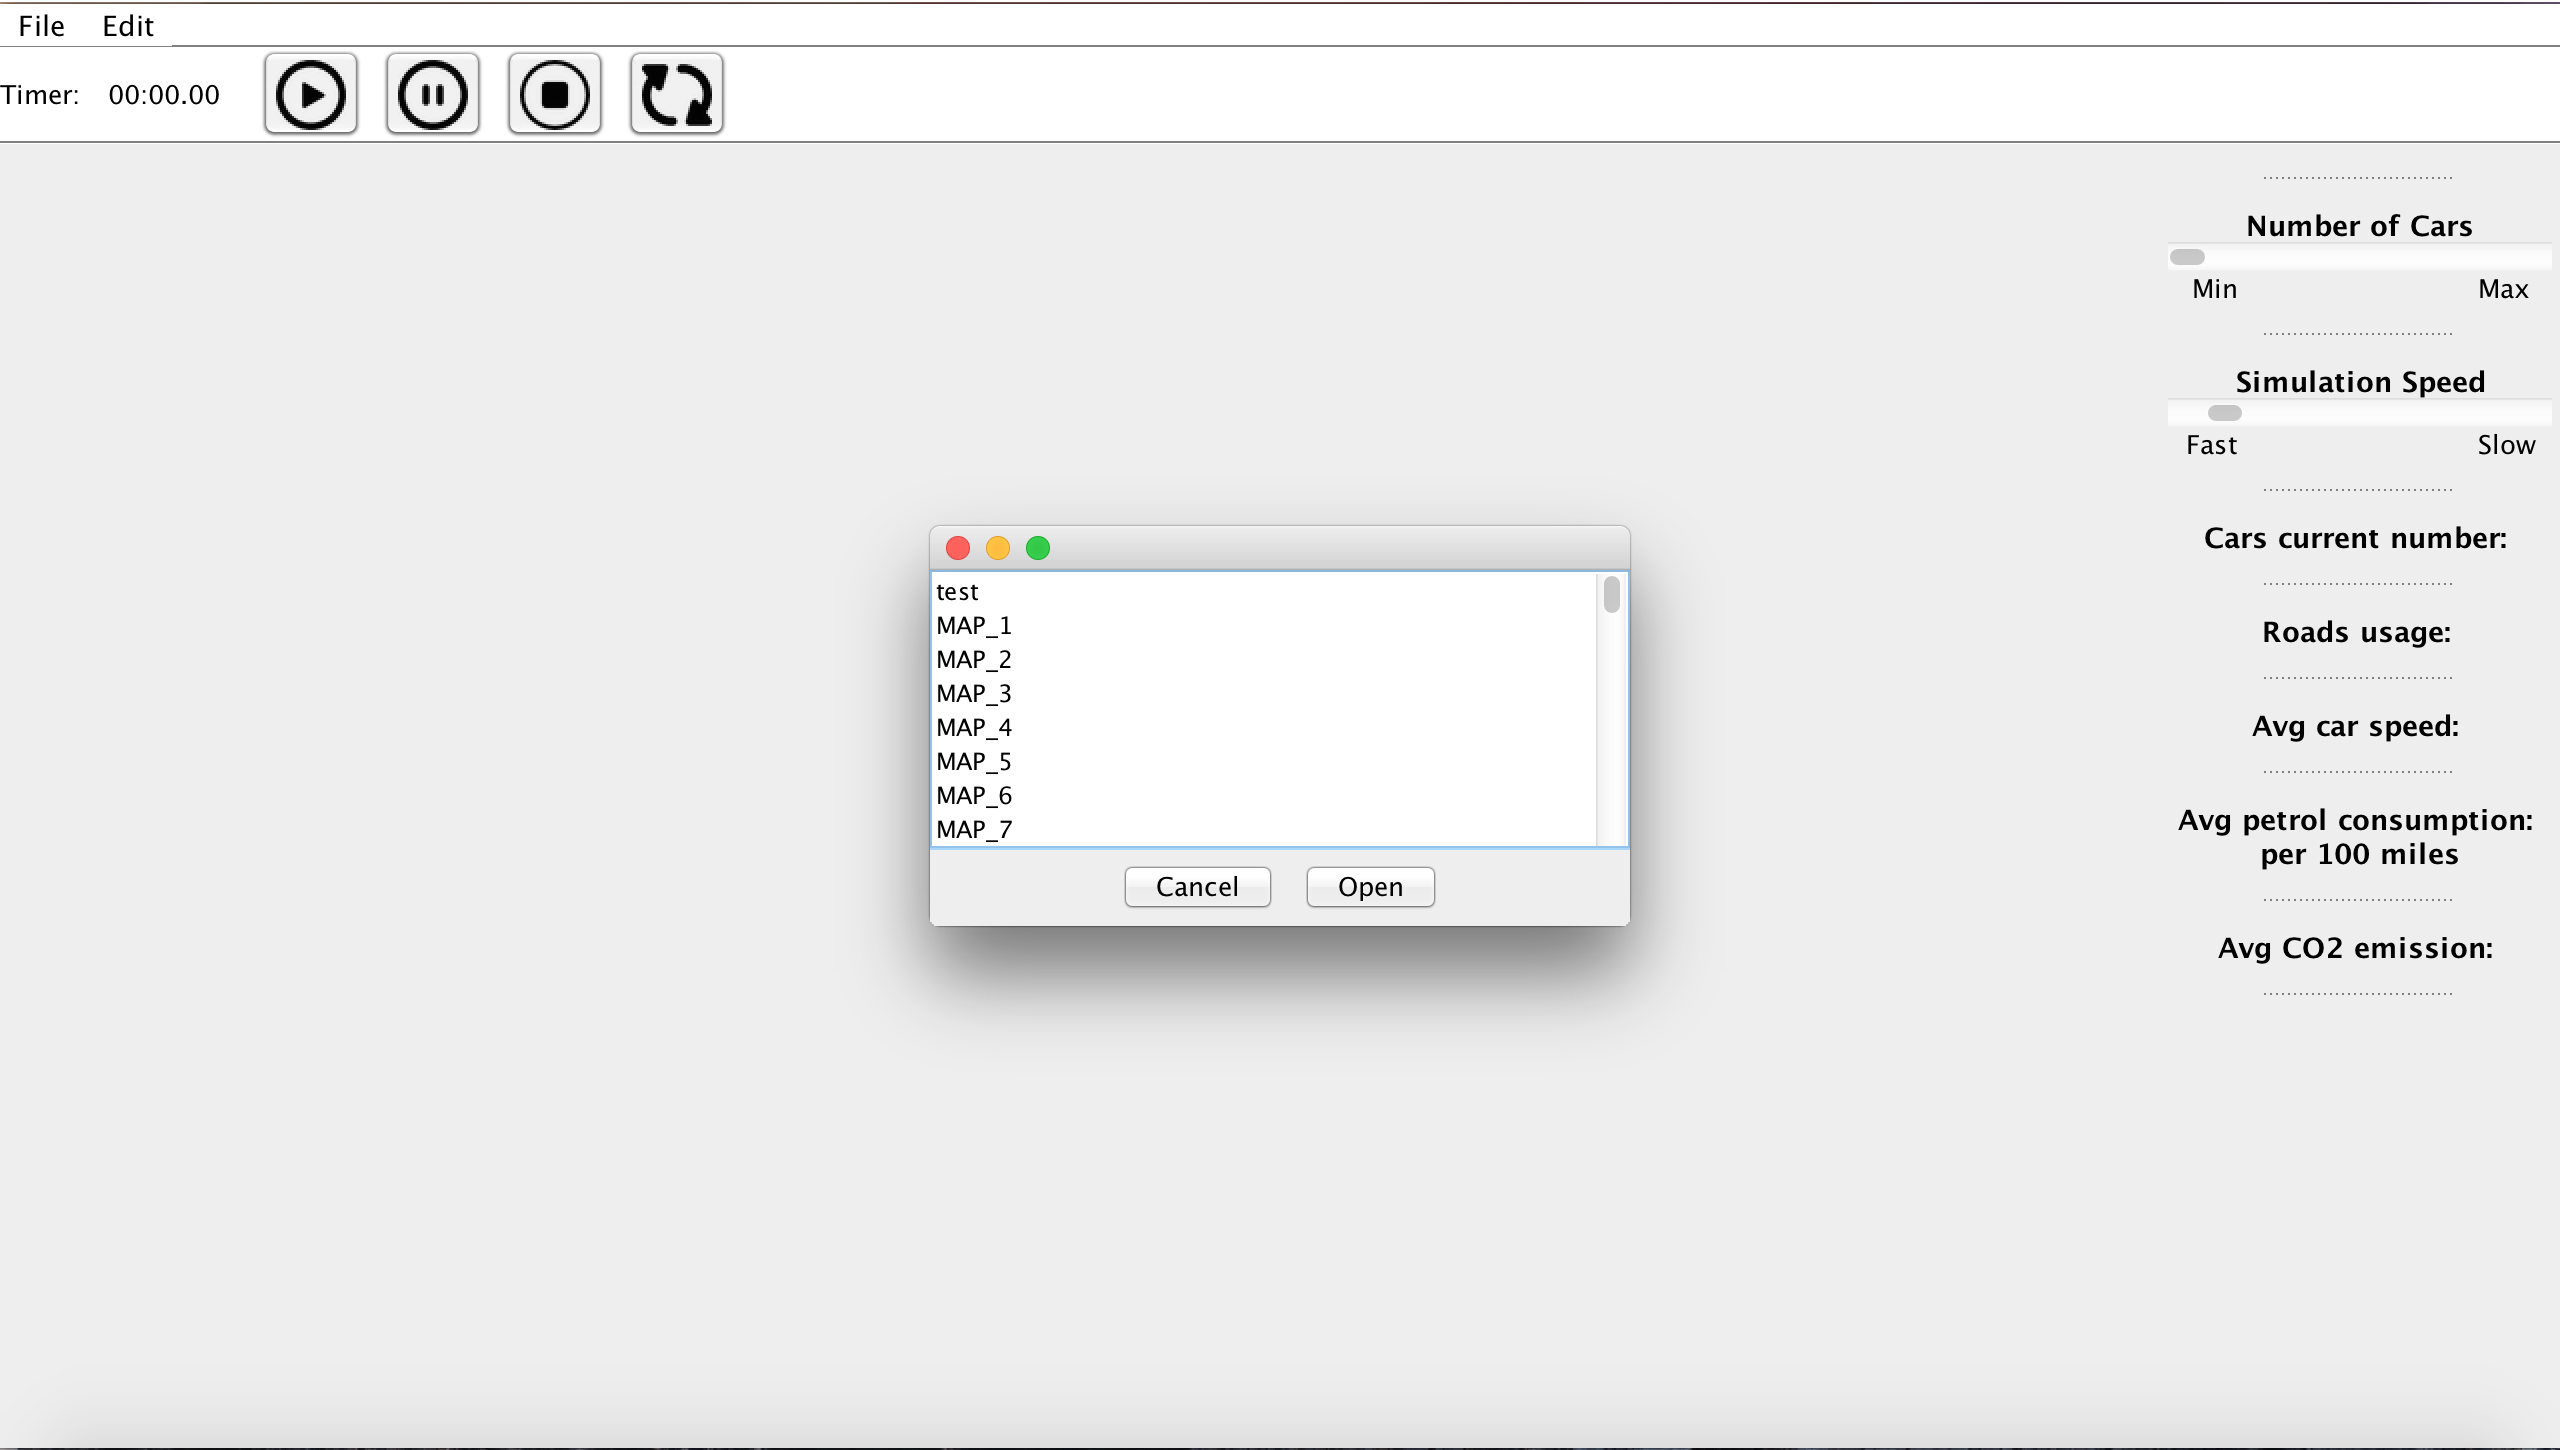
\includegraphics[width=6in]{img4}
\caption{Map Choice} 
\end{figure}

\begin{figure}[h2] 
\centering 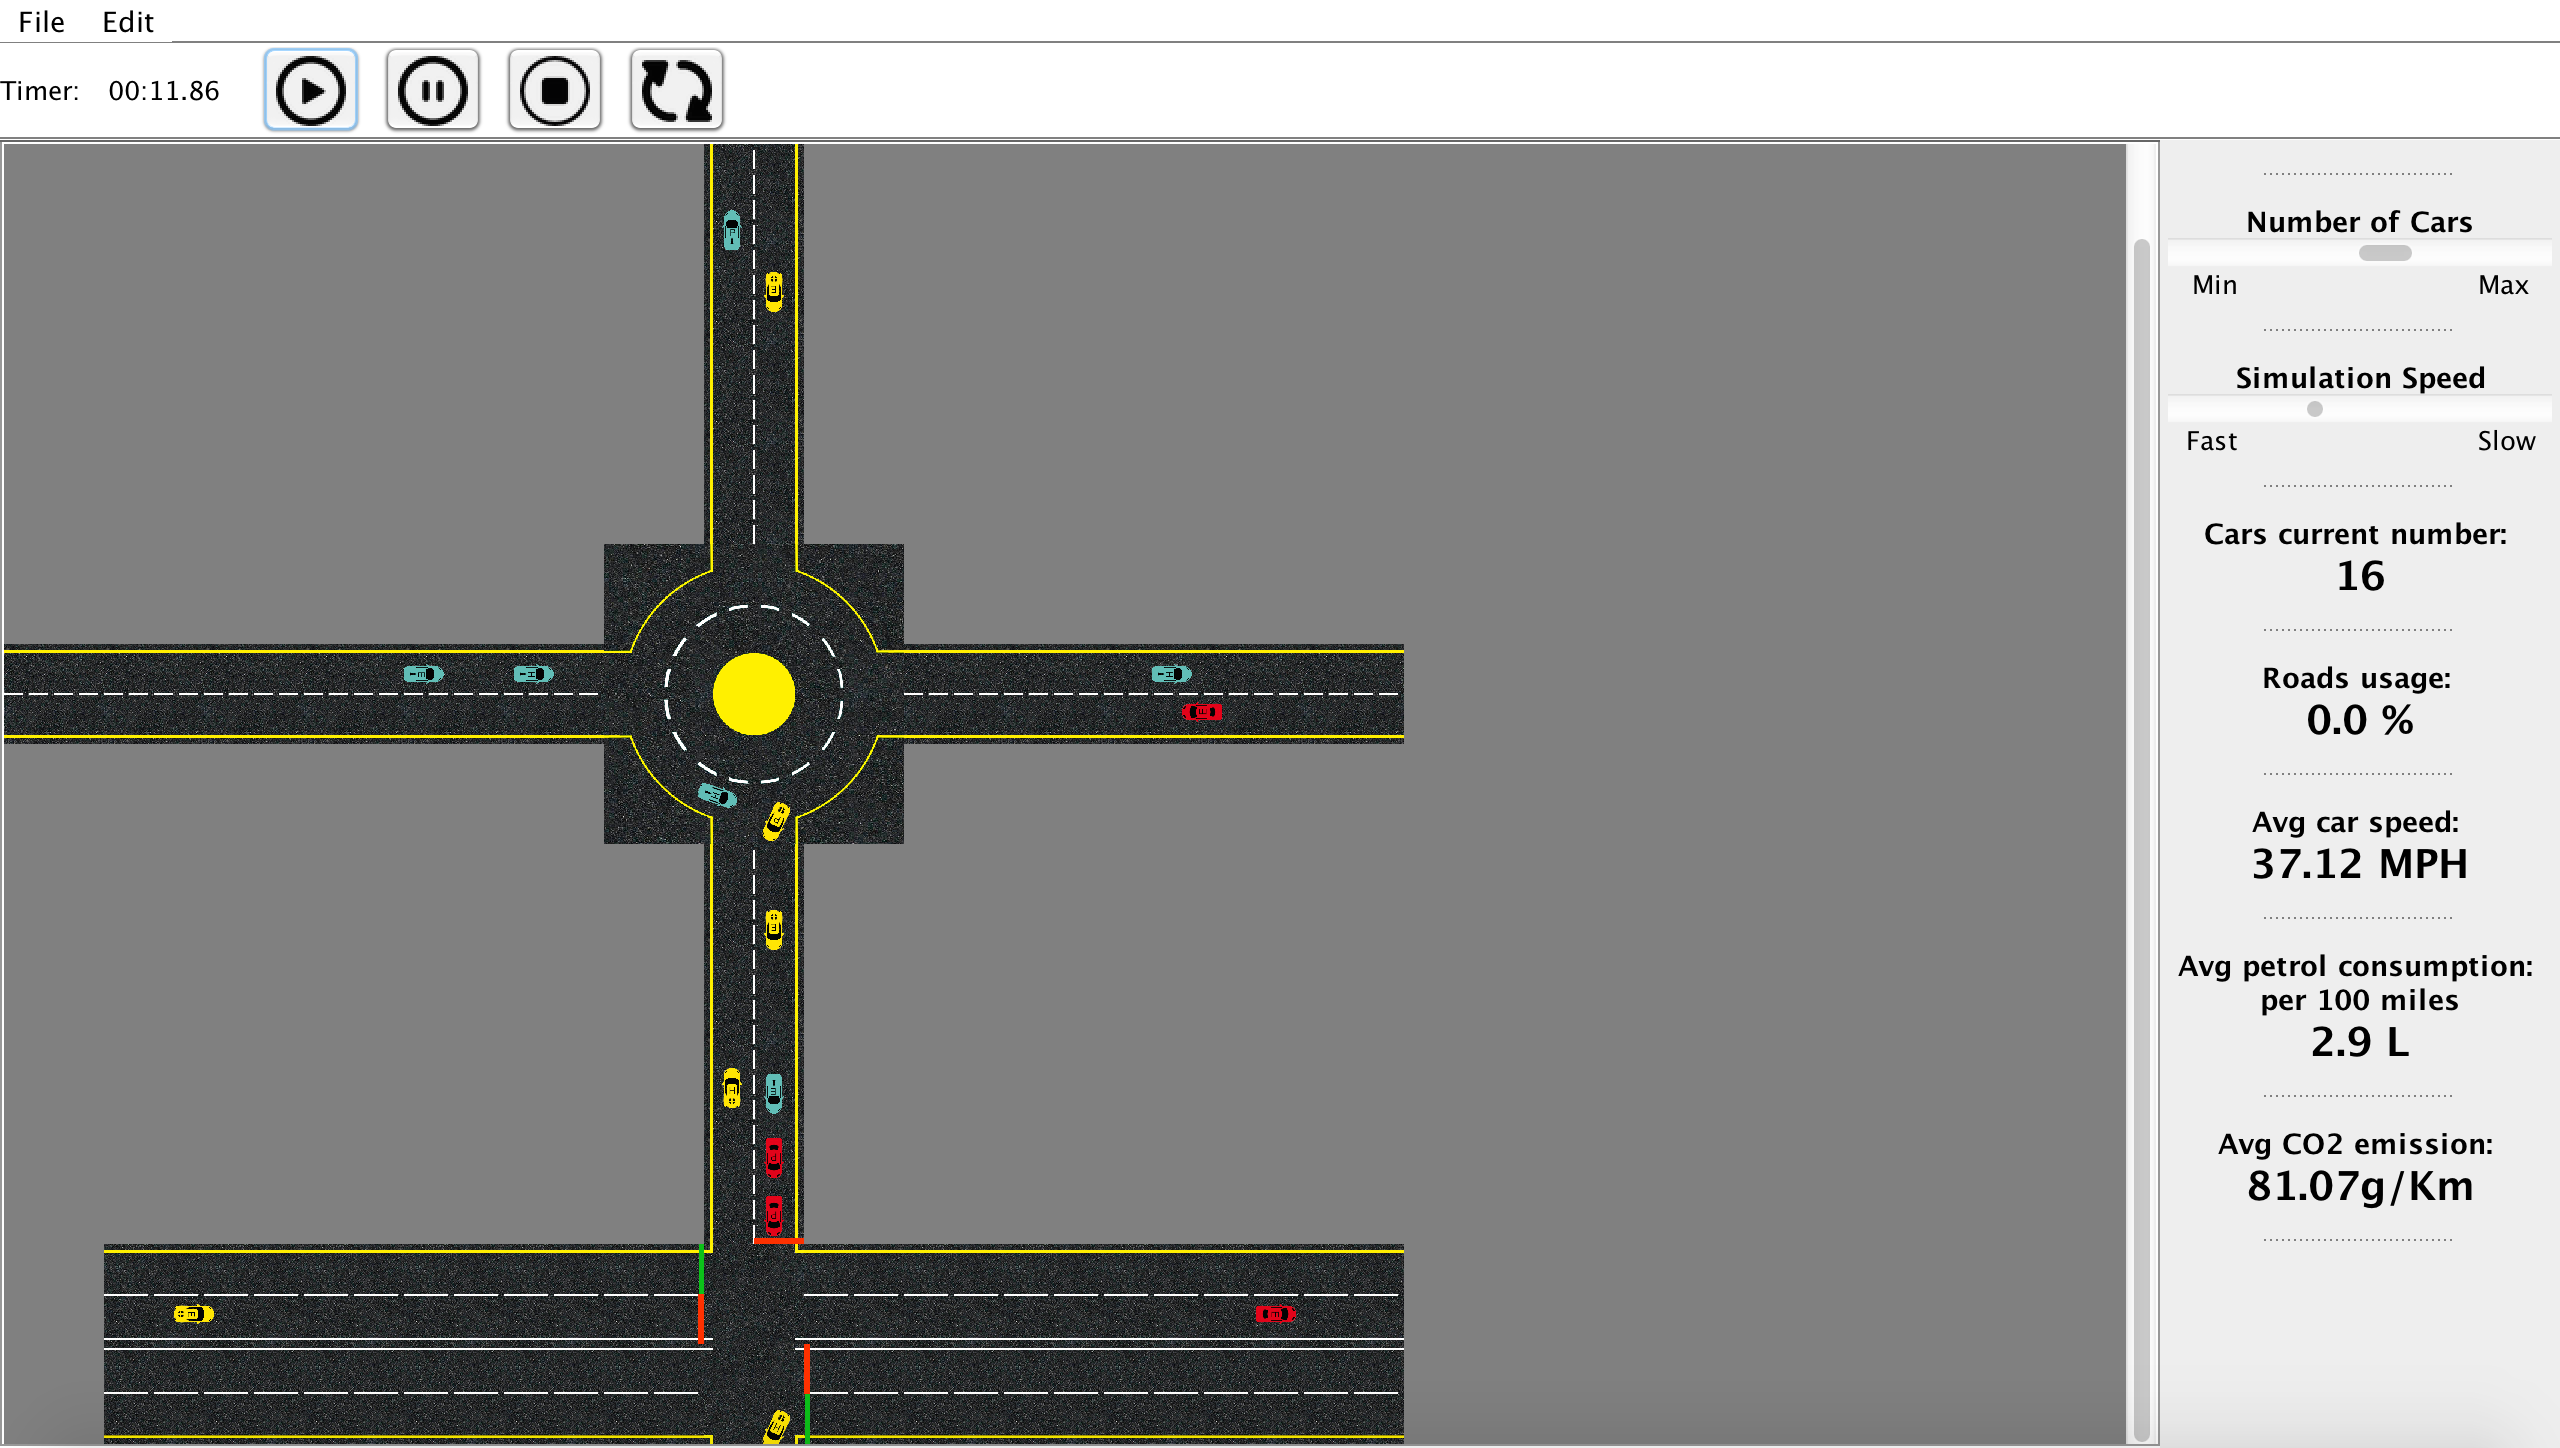
\includegraphics[width=6in]{img5}
\caption{Simulation View} 
\end{figure}


\end{document}
